\documentclass{beamer}
\usepackage[utf8]{inputenc}
% \usepackage{default}
% \usepackage{paralist}
% \usepackage{enumitem}
\usepackage{adjustbox}
\usepackage{changepage}
\usepackage{color, colortbl}
\usepackage{enumerate}
% \setlist{align=left}
\usetheme{Warsaw}
\usecolortheme{beaver}
% \usetheme{Antibes}
% \geometry{paper=a4}
\def\Put(#1,#2)#3{\leavevmode\makebox(0,0){\put(#1,#2){#3}}}
\setbeamertemplate{navigation symbols}{}   
\setbeamertemplate{footline}{}   

\definecolor{Gray}{gray}{0.9}
\definecolor{GrayOscuro}{gray}{0.71}
\definecolor{celestito}{rgb}{0.88,1,1}

\title{Implementación de una herramienta bioinformática para el diseño de secuencias linker}
\date{}

\author{Ignacio Eguinoa}
\institute[VFU] % (optional)
{ Laboratorio de Fisiología de proteínas\\ 
Departamento de Química Biológica \\
Facultad de Ciencias Exactas y Naturales - IQUIBICEN - CONICET\\
Universidad de Buenos Aires}

\begin{document}










% My name is ... 
% 

% I will present PATENA, which is an algorithm for the design of protein linker sequences
% So lets first see why we need a linker sequence....

%*************SWITCH 

% *********************************************
%            MI PRESENTACION
% *********************************************
\begin{frame}
\vspace{20px}
% \hspace{30px}
% 
\includegraphics[width=56px,height=60px]{../img/logo-unlp.jpeg}
% \hspace{62.7px}
% 
\includegraphics[width=70px,height=50px]{../img/logoCONICET.jpg} 
% \hspace{15px}
% 
\includegraphics[width=100px,height=60px]{../img/logoLFP.jpeg}
\titlepage
\end{frame}

















% We want to tag a protein by fusion of a fluorescent protein.
% We known that GFP can provide this (fluorescence) 
% So we decide to use it and we first think a possible construction, made of our target protein(in this case, tubulin), linked to GFP.
% it has been studied that GFP is a relatively small and inert molecule, that doesn't seem to interfere with any biological processes of interest, 
% but the addition of it to can affect the localization or function of the tagged protein
% to prevent this, it is important to use the correct linker sequence, so the whole construction will have the desired properties
% ....OPCIONAL .......  otras coas importantes.....we need to decide if the GFP is added in C or N terminal, that is , the order of the elements....also
\begin{frame}[plain]{Proteínas quiméricas}
\begin{adjustwidth}{-2.0em}{-2.0em}
Usar GFP para marcar una proteína \textit{in vivo}\\
% Use of GFP as fluorescent tag\\
\Put(60,-300){ 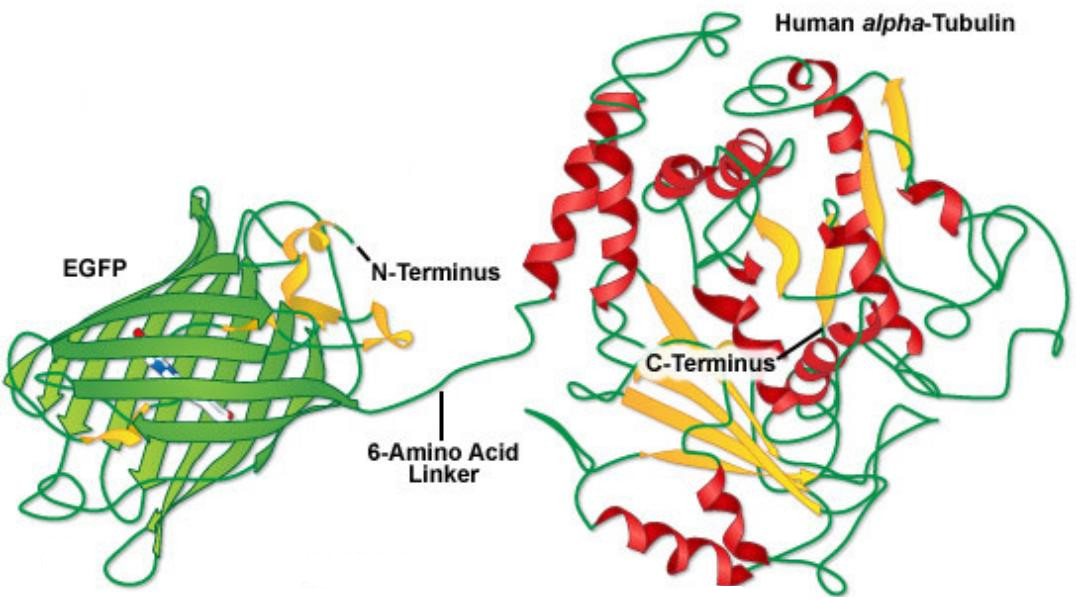
\includegraphics[width=260px]{../img/proteinFusion-GFP-tubulinTransparent.png}}
\\
Construcción: GFP + Linker + Tubulina\\
% Construction: GFP + Linker + Tubulin\\
\vspace{145px}
Al fusionar con GFP podemos estar afectando la localización o funcionalidad de la proteína marcada  $\rightarrow$ \textbf{es importante usar el linker correcto}
% Addition of GFP can affect the localization or function of the tagged protein $\rightarrow$ \textbf{importance of correct linker}
\end{adjustwidth}
\end{frame}














% Second: the sequence needs to adopt a flexible conformation. This propoerty will allow the units to move and interact freely. To provide this flexibility, the sequence . 
% What is more, this property needs to remain constant, so 

% It is also very important that the linker sequence remains biologically inert. That means we dont want any kind of interaction with molecules that could interfere with normal processes of biological system.

% Finally, the linkers will be part of an experimental process, so there can be some other preferences regarding composition, specifically AAs frequencies, UV silent, net charge.

\begin{frame}{Propiedades importantes de un linker}
\vspace{-20px}
\begin{adjustwidth}{-0.5em}{-1.5em}
% \textbf{Allows domains to fold independently, move and interact freely}
\textbf{Secuencia que permite a los dominios plegarse de forma independiente, además de moverse e interaccionar libremente}
\end{adjustwidth}

 \vspace{10px}

\begin{itemize}
  \item Longitud
  \item Mantenga una conformación flexible  %incluye prevencion de aggregation
    \begin{itemize}
     \item Estructura desordenada, no agregada
    \end{itemize}

  \item Biológicamente inerte  %lack of functional features
    \begin{itemize}
     \item No posee interacción alguna con el entorno
    \end{itemize}

  \item Otros aspectos deseables  %experimental aspects
    \begin{itemize}
     \item Frecuencias de aminoácidos, silente en UV, carga neta
\end{itemize}
\end{itemize}
\end{frame}









% At the moment we have 3 different approaches to linker design
% First we can, of course, use linkers extracted from natural multidomain proteins
% We can also propose novel designs containing small and disorder-favoring(disorder-promoting) amino acids.
% Another option is to use different servers available. These servers collect natural and aritificial linkers and provide a search over these set using specific parameters, so the user can find a sequence with the required properties
% (length,    ....)

% We will be able to get different designs but...    , 
% most of the sequences we will get wont have all the desired properties. 
% for example, natural linkers can, of course, have biological functions
% others can have rigid structure
% even if we get sequences with all desired properties, the set of possible designs will be very small, and we will only get a few possible different designs.



\begin{frame}{Métodos actuales de diseño}
\begin{itemize}

% \item Use linkers from natural multi-domain proteins
\item Usar linkers de proteínas multidominio naturales

\item Diseños intuitivos
 \begin{itemize}
  \item Generalmente ricos en G-S-P 
  \end{itemize}
\item Aproximaciones Pseudoracionales. 
\begin{itemize}
 \item Servidores: LINKER, Linkerdb, SynLinker.
\end{itemize}
\end{itemize}
\vspace{20px}
\LARGE{Estructurados? Inertes? Diversos?}
\end{frame}













% Clearly, we dont have a method to design linkers with the correct properties
% but if we have a sequence, we can check any undesired feature by means of different bioinformatic tools available, that can analyze the sequence
% That is, We can predict all unwanted properties.
% OPTIONAL ...That is, we can evaluate (get an idea, get an estimation of) how good or how bad(quality) is a sequence to work as a linker.

% ACA PRESENTO LAS HERRAMIENTAS DE FORMA INDIVIDUAL
% PARA CADA HERRAMIENTA PRESENTADA DECIR QUE LO QUE HARIA ES AGARRAR MANUALMENTE LA SECUENCIA, USAR LA HERRAMIENTA Y ANALIZAR SI TIENE ALGUNA PROPIEDAD INDESEADA


\begin{frame}{Evaluación de la secuencia}

Teniendo una secuencia candidato:\\
\begin{itemize}
 \item Existen diferentes herramientas bioinformáticas para predecir propiedades no deseadas. % a partir del analisis de las propiedades no deseadas
\end{itemize}

% 
% ACÁ SIGO CON UNA DESCRIPCION MUY BREVE DE LOS MÉTODOS MAS IMPORTANTES DE  EVALUACION QUE USAMOS
% SIEMPRE INDICANDO QUE AGARRO LA SECUENCIA USO ESE METODO Y OBTENDO LA PRESENCIA DE BLA BLA
 
% \vspace{10px}
\pause
\begin{block}{IUPred}
Permite estimar un potencial de interacción para cada residuo de la secuencia, de acuerdo al contexto en el que se encuentra.
% por ejemplo, si quiero saber si la secuencia tiene una tendencia a adoptar una conformacion globular, algo que no queremos, puedo usar la herramienta iupred que hace bla bla 
% me paermite para cada posicion estimar un potencial de interaccion de acuerdo al contexto en el que se encuentra ese residuo en la secuencia, y si es posible 
% IUPRED
% 	Modelo parametrizado usando bases de datos de estructuras globulares
% 	Estimar un potencial de interacción basado en la composición de aminoácidos de la secuencia.
% 	No requiere conocer/asumir una conformación.
% 	Efecto secundario: elimino funciones biológicas que requieran una estructura concreta.
\end{block}
% 
% 
% \end{frame}

\pause
% \begin{frame}
\begin{block}{BLAST}
 Permite inferir funcionalidades biológicas a partir de similitud secuencial.
\end{block}
\pause
\begin{block}{ELM}
% \begin{itemize}
 Permite buscar instancias de motivos lineales cortos en la secuencia.
%  \item Recopilación de motivos lineales curados manualmente de la literatura
% \end{itemize}
% Hay algunos elementos funcionales que suelen encontrarse en regiones desordenadas que suelen llamarse motivos lineales cortos. 
% Estos están anotados en el resucrso ELM.  la idea de este recurso es que, como son elementos cortos y son difificiles de encontrar por métodos de similitud , 
% se recopilan manualmente estos elementos de la literatura y se guardan en una base de datos en forma de patrones. 
% Podemos buscar instancias de estos patrones en nuestra secuencia, para saber si es posible que tenga alguna funcionalidad asociada a estos motivos lineales.
\end{block}

\end{frame}





\begin{frame}

\begin{block}{ANCHOR}
% \begin{itemize}
%  \item  Segmentos que se encuentran normalmente desordenados pero pueden adquirir una estructura al ligarse a moléculas específicas. 
 Extiende el modelo de IUPred para estimar la ganancia de energía que tendrá el segmento en un contexto de cierta composición determinada.
% \end{itemize}
\end{block}

\pause
\begin{block}{PASTA}
\begin{itemize}
 \item Asume que las interacciones en la formación de estructuras \textit{cross-$\beta$} es el mismo que en las estructuras de $\beta$-sheets.
 \item Deriva un potencial estadístico de interacción entre cada par posible de AAs en este tipo de estructura.
 \item Se evaluan todos los posibles emparejamientos de la secuencia con si misma.
%  \item El emparejamiento que tenga menor energia asignada se predice como el que se adopará en caso que se forme el agregado de tipo amiloide.
\end{itemize}
\end{block}

% % BLAST
% % 	Buscar similitudes secuenciales que puedan indicar una funcionalidad. 
% % 	En particular blast permite buscar eficientemente similitudes secuenciales en una gran base de datos. Si bien es heuristico
% % 	Hay que tener en cuenta:
% %	 	Matches Vs no-matches.
% % 		Solo se tiene en cuenta el primer hit. Cutoff? 
% 
\end{frame}






















% ENTONCES SABEMOS QUE PODEMOS HACER UN ANALISIS MANUAL DE QUE TAN BUENO ES UN LINKER ANALIZANDO INTIVIDUALMENTE LA PRESENCIA DE ELEMENTOS NO DESEADOS
% En resumen, el set de evaluaciones queda definido por: 
% IUPred, to evalute if the sequence will adopt a globular structure
% we have 3 different methods to evaluate sequence propensity to form insluble aggregates
% functional features are evaluated by means of: BLAST(to try to infer function through sequence similarity), also  ELM resource(to find instances of linear motifs), PROSITE(to find functional sites), and ANCHOR(to find recognition elements)
% Finally, some optional evaluations are:
%      check the presence of ultraviolet aboserbers aminoacids W(Tryptophan), Y(Tyrosine), F(Phenylalanine)
% 	and check the presence of charged residues.


% so....what do we do with this evaluation set?
% ESTE CONJUNTO DE HERRAMIENTAS INDIVIDUALES LAS USO DE FORMA ESTANDARIZADA EN UN MECANISMO DE EVALUACION DE SECUENCIAS CANDIDATO, (esta estandarizacion implica fijar valores de cutoff, mecanismos para definir positivos/negativos, etc)
% Y ESTO ES EL NUCLEO DE NUESTRA HERRAMIENTA

% 
% DECIR QUE TODOS LOS MÉTODOS DAN INFORMACION A NIVEL DE POSICION DENTRO DE LA SECUENCIA
%  any of these methods allows to define if a particular position contains a specific negative aspect 
% each of these methods allows to asses if a particular position has that specific negative aspect we are evaluating
% so we can define a scoring function

\begin{frame}{Aproximación racional}
 

Cada uno de estos métodos permite predecir la presencia de alguna característica no deseada en posiciones específicas $\rightarrow$ definir una función de puntuación.
\vspace{10px}

% Como primer paso para el desarrollo de un método de diseño racional
\begin{itemize}
 \item Definimos un conjunto completo de métodos para predecir la ocurrencia de propiedades indeseadas en la secuencia candidato a linker.
\end{itemize}

\vspace{10px} 

\begin{adjustbox}{width=\textwidth}
\begin{tabular}{l|l}
\textbf{Características no deseadas} & \textbf{Método de predicción} \\ \hline \hline
\rowcolor{Gray} Estructura globular & IUPred, TMHMM \\
Agregados insolubles  & TANGO, PASTA, WALTZ   \\
\rowcolor{Gray}Características funcionales & BLAST, ELM, PROSITE, ANCHOR, Limbo \\  
Absorción UV (opcional) & W, Y, F \\ %Presence of UV-absorbers residues \\
\rowcolor{Gray}Carga neta (opcional)& Presencia de residuos cargados\\
\end{tabular}
\end{adjustbox}

\vspace{10px}
\begin{itemize}
 \item Interpretamos los resultados como valores binarios 
\end{itemize}

\end{frame}




























% this is an example of application of this scoring function
% each tool provides a value of 1 for each position that has undesired feature. 
% summing up all the values for each position we have a position score, defining the total number of undesired features for it
% and finally, if we add all the position scores we can get a global score.
% so we have a function, defining a value of how bad is a linker. what can we do with it? ..... ****SWITCH

% *********************************************
%      EJEMPLO DE EVALUACION DE SCORE
% *********************************************
% 
\begin{frame}{Ejemplo de evaluación}

\begin{adjustbox}{width=\textwidth}
 \begin{tabular}{llllllllllllll} 
\hline
\rowcolor{GrayOscuro}Secuencia & \textbf{M} & \textbf{V} & \textbf{L} & \textbf{S} & \textbf{P} & \textbf{A} & \textbf{D} & \textbf{K} & \textbf{T} & \textbf{N} & \textbf{P} & \textbf{D} \\ \hline \hline
 
% Puntaje Inicial & 0 & 0 & 0 & 0 & 0 & 0 & 0 & 0 & 0 & 0 & 0 & 0\\ \hline
\rowcolor{Gray}IUPred           	& 0 & 1 & 1 & 1 & 1 & 0 & 0 & 1 & 1 & 1 & 0 & 0\\ \hline  
TANGO 		       			& 1 & 1 & 1 & 1 & 0 & 0 & 0 & 0 & 0 & 0 & 0 & 0\\ \hline  
\rowcolor{Gray}PASTA			& 1 & 1 & 0 & 0 & 0 & 0 & 0 & 1 & 0 & 1 & 1 & 1\\ \hline  
ELM          	      			& 0 & 1 & 1 & 0 & 0 & 0 & 0 & 1 & 1 & 1 & 1 & 1\\ \hline 
\rowcolor{Gray}BLAST			& 1 & 0 & 1 & 1 & 1 & 0 & 0 & 0 & 0 & 1 & 1 & 1\\ \hline 
PROSITE 	      			& 0 & 0 & 1 & 0 & 0 & 0 & 0 & 0 & 0 & 1 & 1 & 1\\ \hline 
\rowcolor{Gray}ANCHOR	        	& 1 & 1 & 1 & 0 & 0 & 0 & 0 & 0 & 0 & 1 & 0 & 1\\ \hline
TMHMM 	      				& 0 & 0 & 1 & 1 & 1 & 0 & 1 & 1 & 1 & 1 & 1 & 0\\ \hline 
\rowcolor{Gray}WALTZ 	      		& 0 & 0 & 1 & 0 & 0 & 0 & 0 & 0 & 0 & 1 & 1 & 1\\ \hline 
Limbo	      				& 0 & 0 & 0 & 0 & 0 & 0 & 0 & 0 & 1 & 1 & 1 & 1\\ \hline \hline 
% REVISAR LAS SUMAS Y VALORES DE LOS ULTIMOS 3
\rowcolor{GrayOscuro}Puntaje posición     & 4 & 5 & 8 & 4 & 3 & 0 & 1 & 4 & 4 & 9 & 7 & 7\\ \hline
\rowcolor{GrayOscuro}Puntaje global  & 56 &&&&&&&&&&& \\ \hline
\end{tabular}
\end{adjustbox}
\end{frame}








% So, we have seen the core of PATENA, x`which is the use of a scoring function to evaluate undesired features of linker sequences
% We now will see how PATENA use this function to implement a linker design method.

% to use this method the user will need to provide a candidate linker , or just the length. 

% as a result, the user will get a sequence which has no undesired features. that is, a sequence with score equal to zero.
% this resulting design can be used as linker

% As you can see, if the user only defines the length of the sequence, this method can design a linker from scratch. 

% lets see more in detail how this method works, using the scoring function to implement an optimization method


\begin{frame}{Método: Input - Output}

% UTILIZANDO EL ESQUEMA DE EVALUACION PREVIO, 
% IMPLEMENTAMOS UN MÉTODO CON EL OBJETIVO DE PODER OBTENER UN DISEÑO FINAL QUE PUEDA SER UTILIZADO COMO LINKER:

% \centering
\vspace{24px}
\begin{adjustwidth}{-2.0em}{-2.0em}
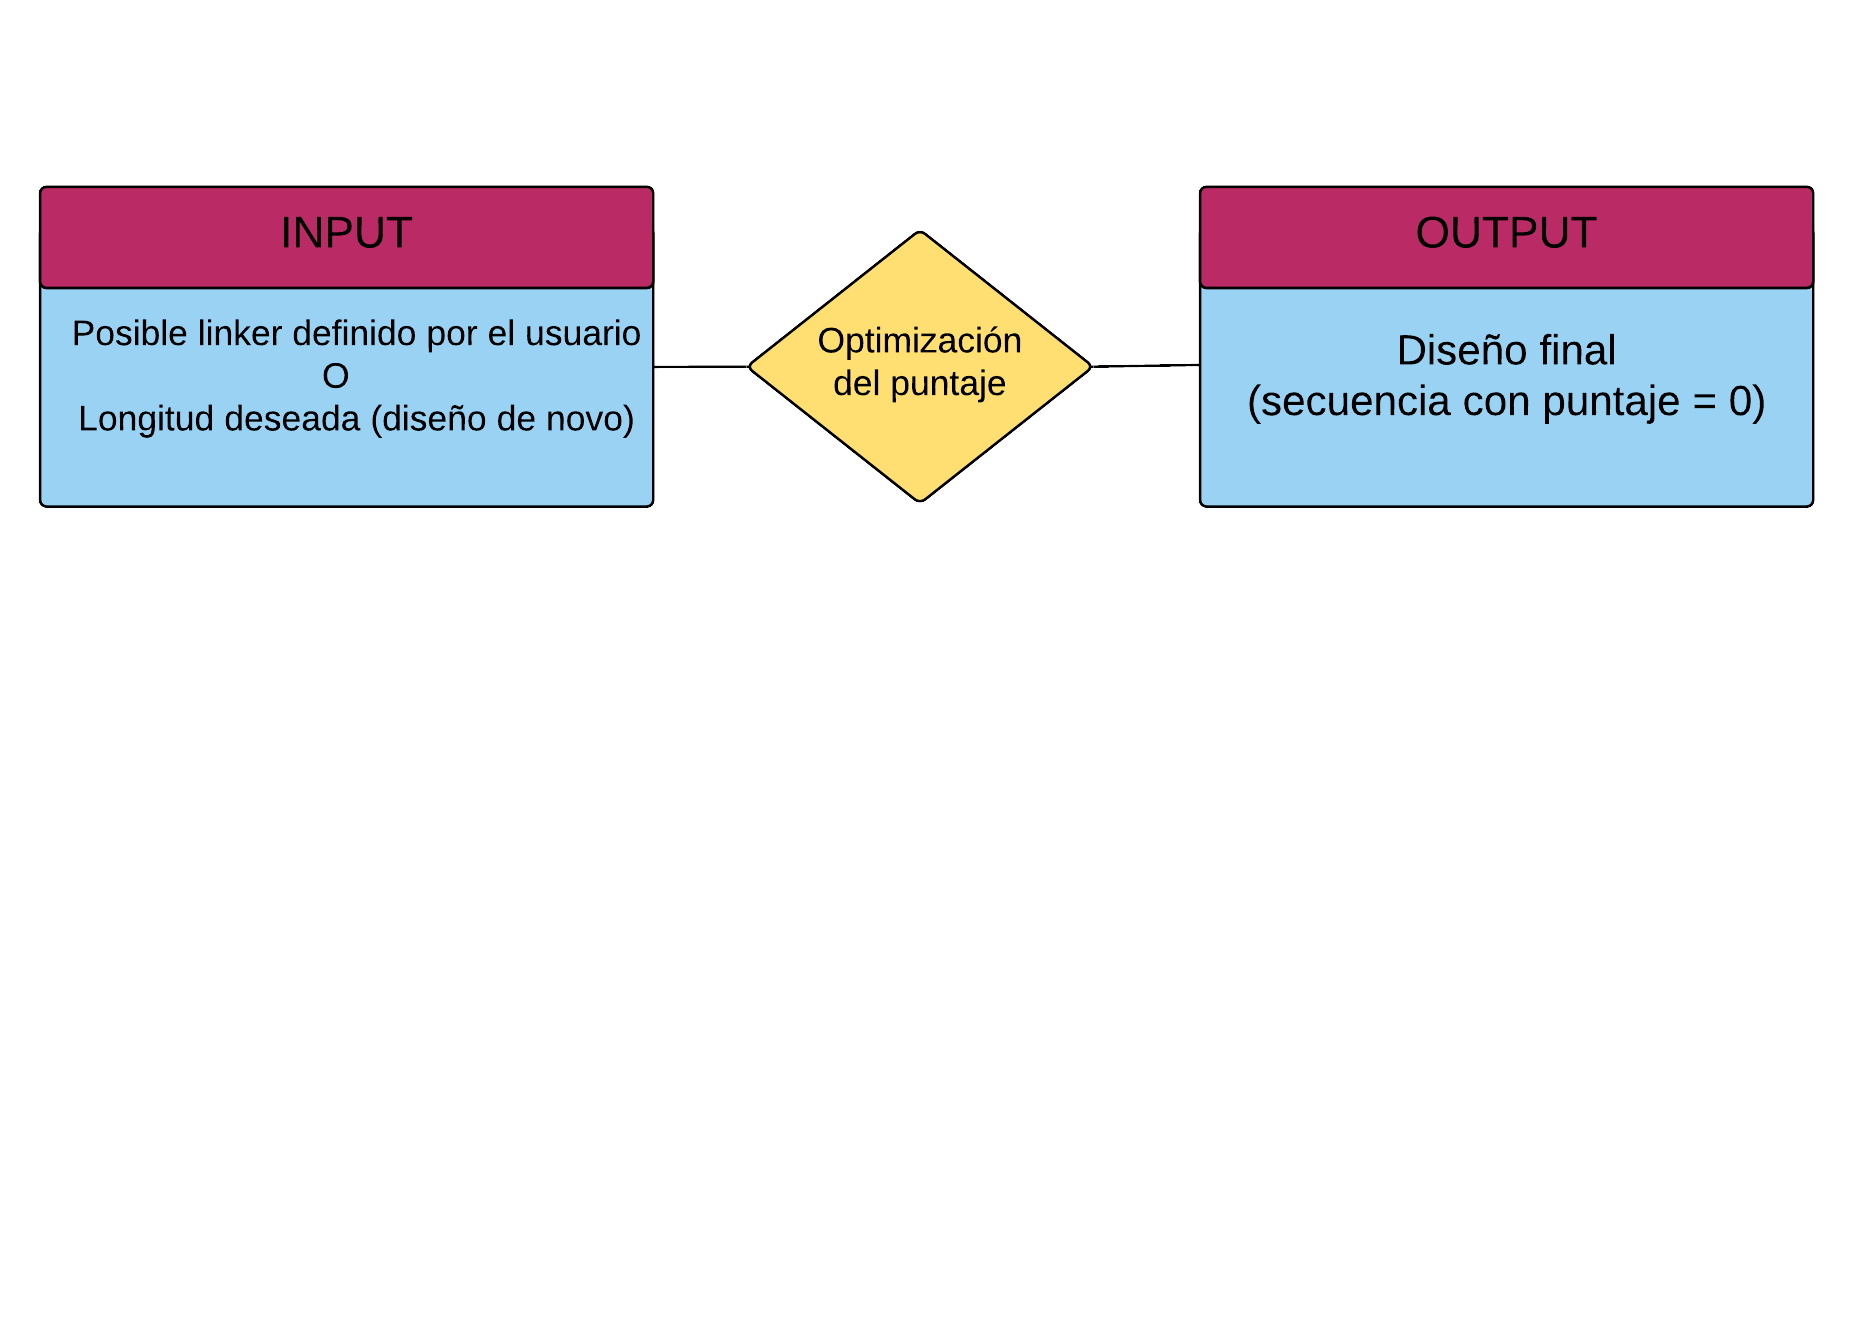
\includegraphics[width=350px]{../img/coarseGrainedPatena-Spanish.png}
\end{adjustwidth}

% EL METODO, BASICAMENTE, PERMITE INICIAR EL DISEÑO DESDE UNA SECUENCIA DEFINIDA POR EL USUARIO O PUEDE EMPEZAR DESDE UNA SECUENCIA RANDOM. EN ESE CASO EL USUARIO SOLAMENTE TIENE QUE DEFINIR LA LONGITUD
% UNA VEZ QUE SE TIENE UNA SECUENCIA INICIAL, USANDO LA FUNCION DE PUNTUACION QUE VIMOS, 

\end{frame}







% The method starts defining an initial sequence, this sequence can be a users input, or if the user defined a length, a random sequence is created.
% Once we have a starting sequence, we make a first score evaluation.
% If the score is greater than zero, we have some undesired features, in this case we propose a point mutation, aiming at the high scoring positions, that is, the positions that accumulate most undesired features.
% We evaluate this proposition, again using the scoring function.
% If this mutation decreases the score, then we will incorporate that into the sequence.
% The heuristic decision is implemented using a method known as Monte Carlo decision. This decision is based on the score difference and on a beta parameter, which is proportional to the acceptance rate.
% Based on this decision we can accept the mutation or not.


% What we have here is, again, an optimization of the scoring function.
% Once we have this algorithm implemented we need to see if we can find an effective beta value that will allow the execution to efficiently find a design.


% *********************************************
%      ESQUEMA GRAFICO DE PATENA
% *********************************************
\begin{frame}[plain]{Esquema del método}
\vspace{-1.0\baselineskip}
\begin{adjustwidth}{-2.0em}{-2.0em}
% \begin{adjustheight}{-1.5em}{-1.5em}
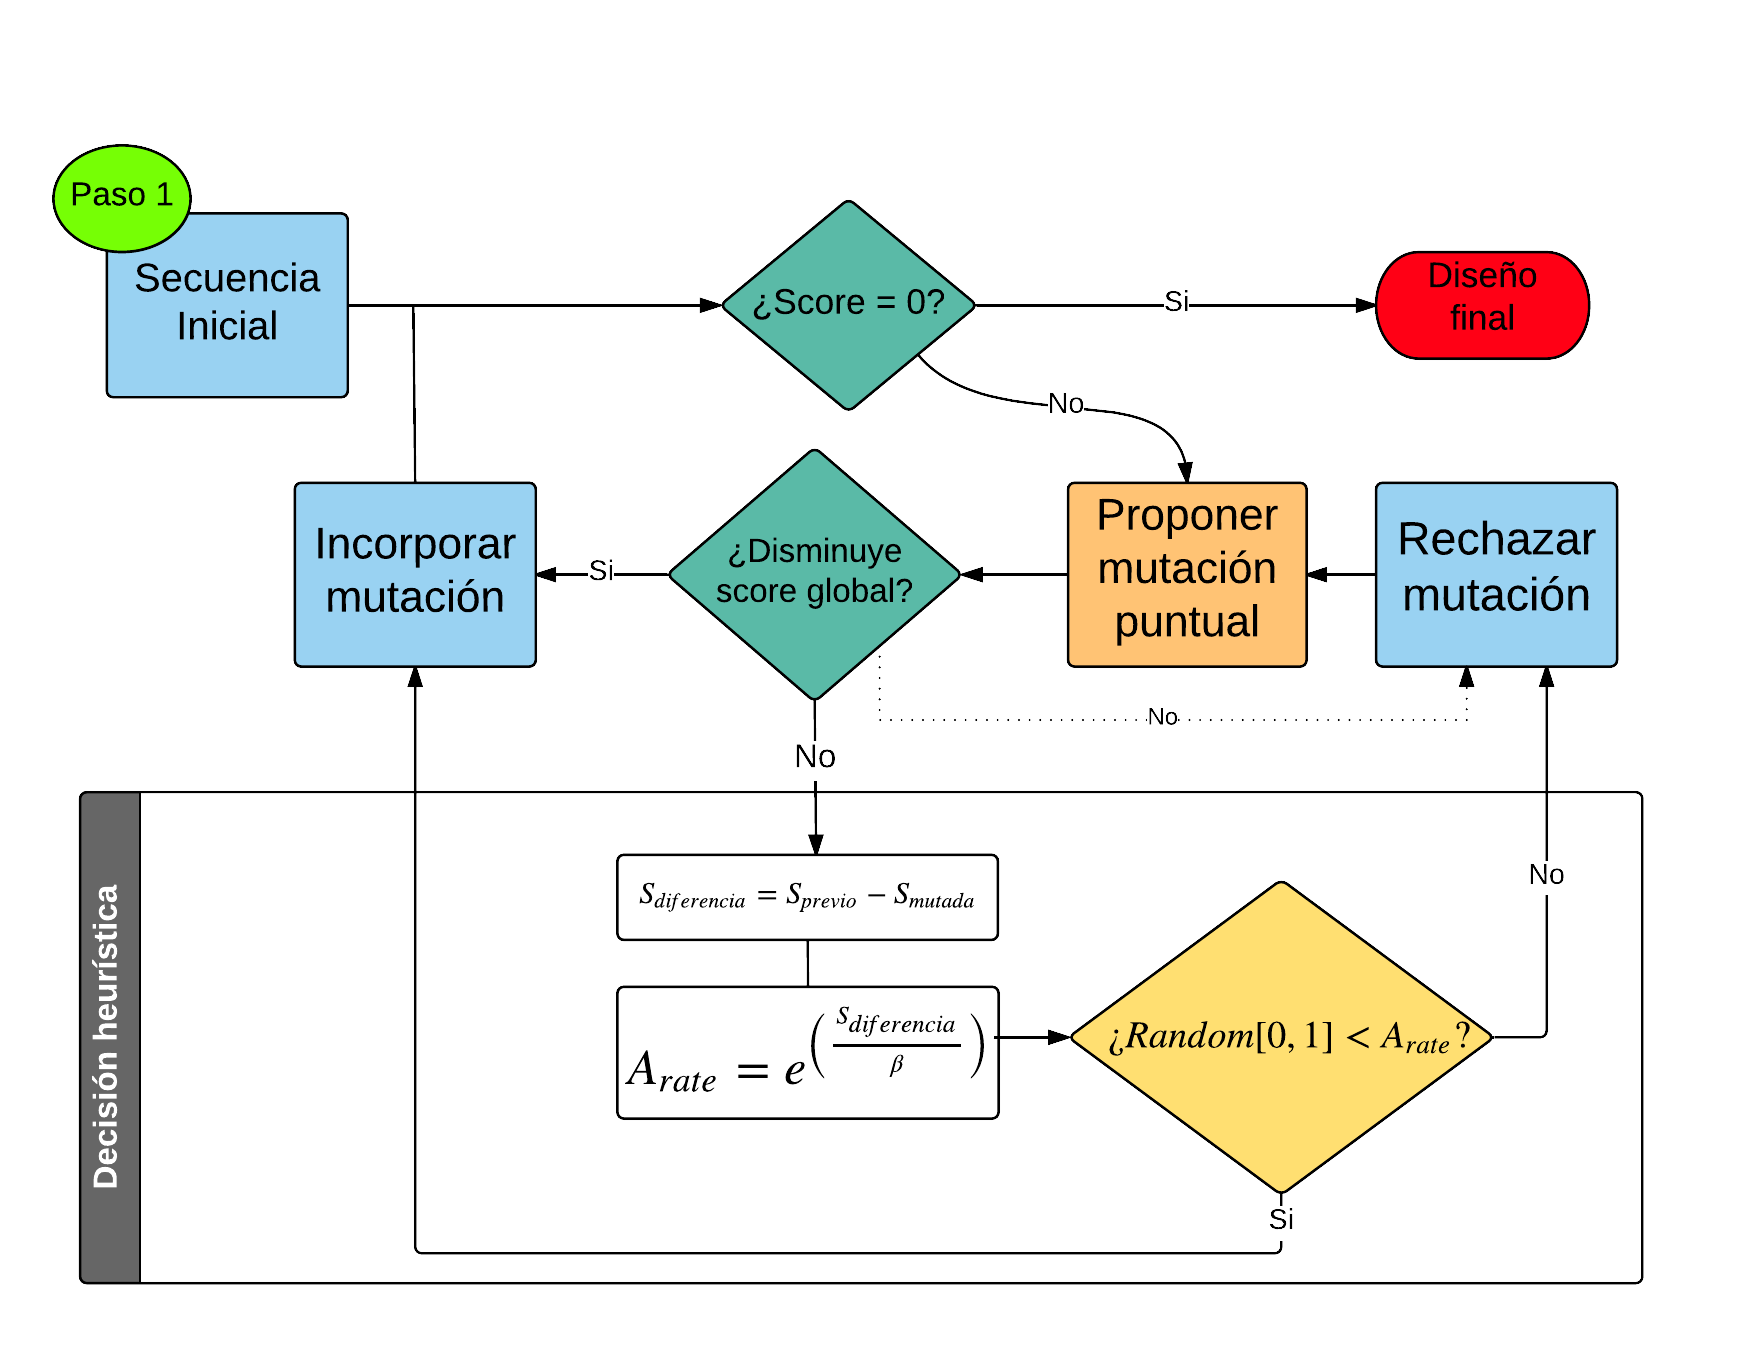
\includegraphics[width=350px,height=250px]{../img/patenaSpanish.png} 
% 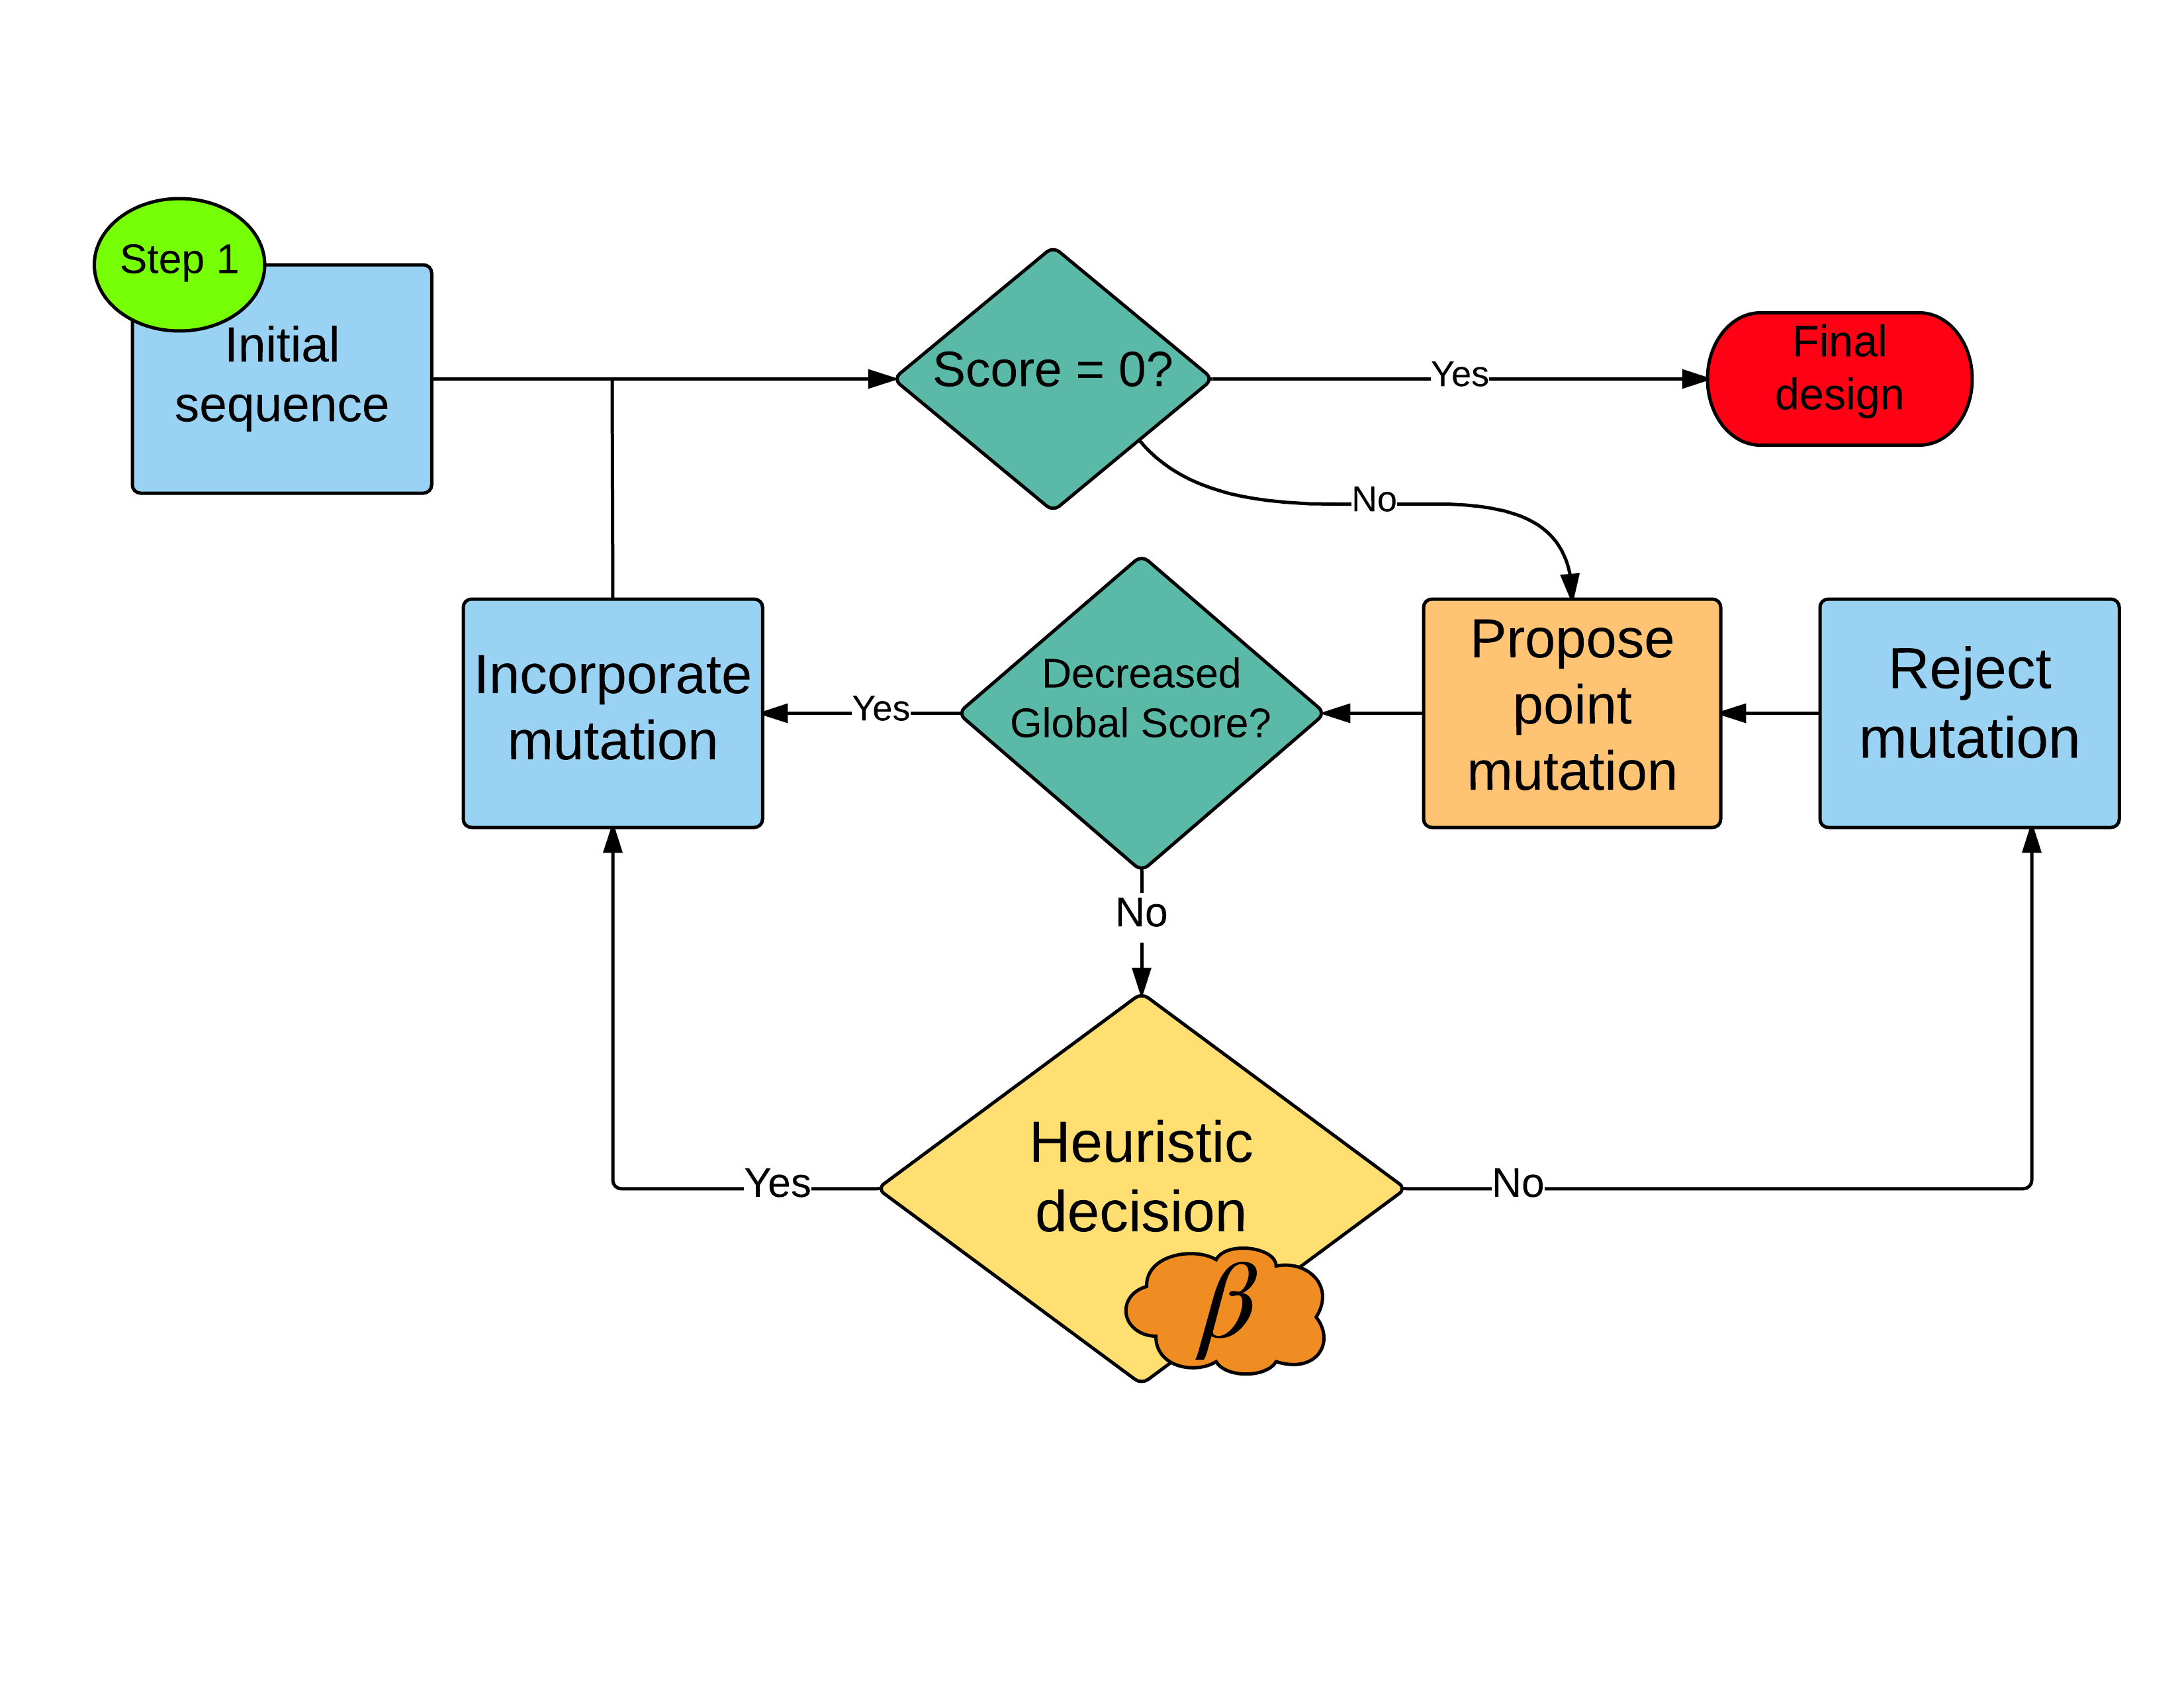
\includegraphics[width=350px,height=250px]{../img/patenaReduced-Beta.png} 
% \end{adjustheight}
\end{adjustwidth}
% \vspace{-\baselineskip}
\end{frame}


























% 
%

% The execution can find designs in all cases but we see that the effective range is located below  beta value of 2.0
% Just to move on with evaluation we choose a beta of 1.0, which is in the middle. This is just a decision we made.

% *********************************************
%      BETA vs TIME
% *********************************************
\begin{frame}[plain]{Rango efectivo de $\beta$ $\approx$ [0.1 - 2.0]}
% Effective $\beta$ range $\approx$ [0.1 - 2.0]}
\centering
% Optimal $\beta$ range  
[Largo = 50] - [Random (n=3) y Naturales (n=3) / cada $\beta$] \\
\begin{adjustwidth}{-1.5em}{-2.5em}
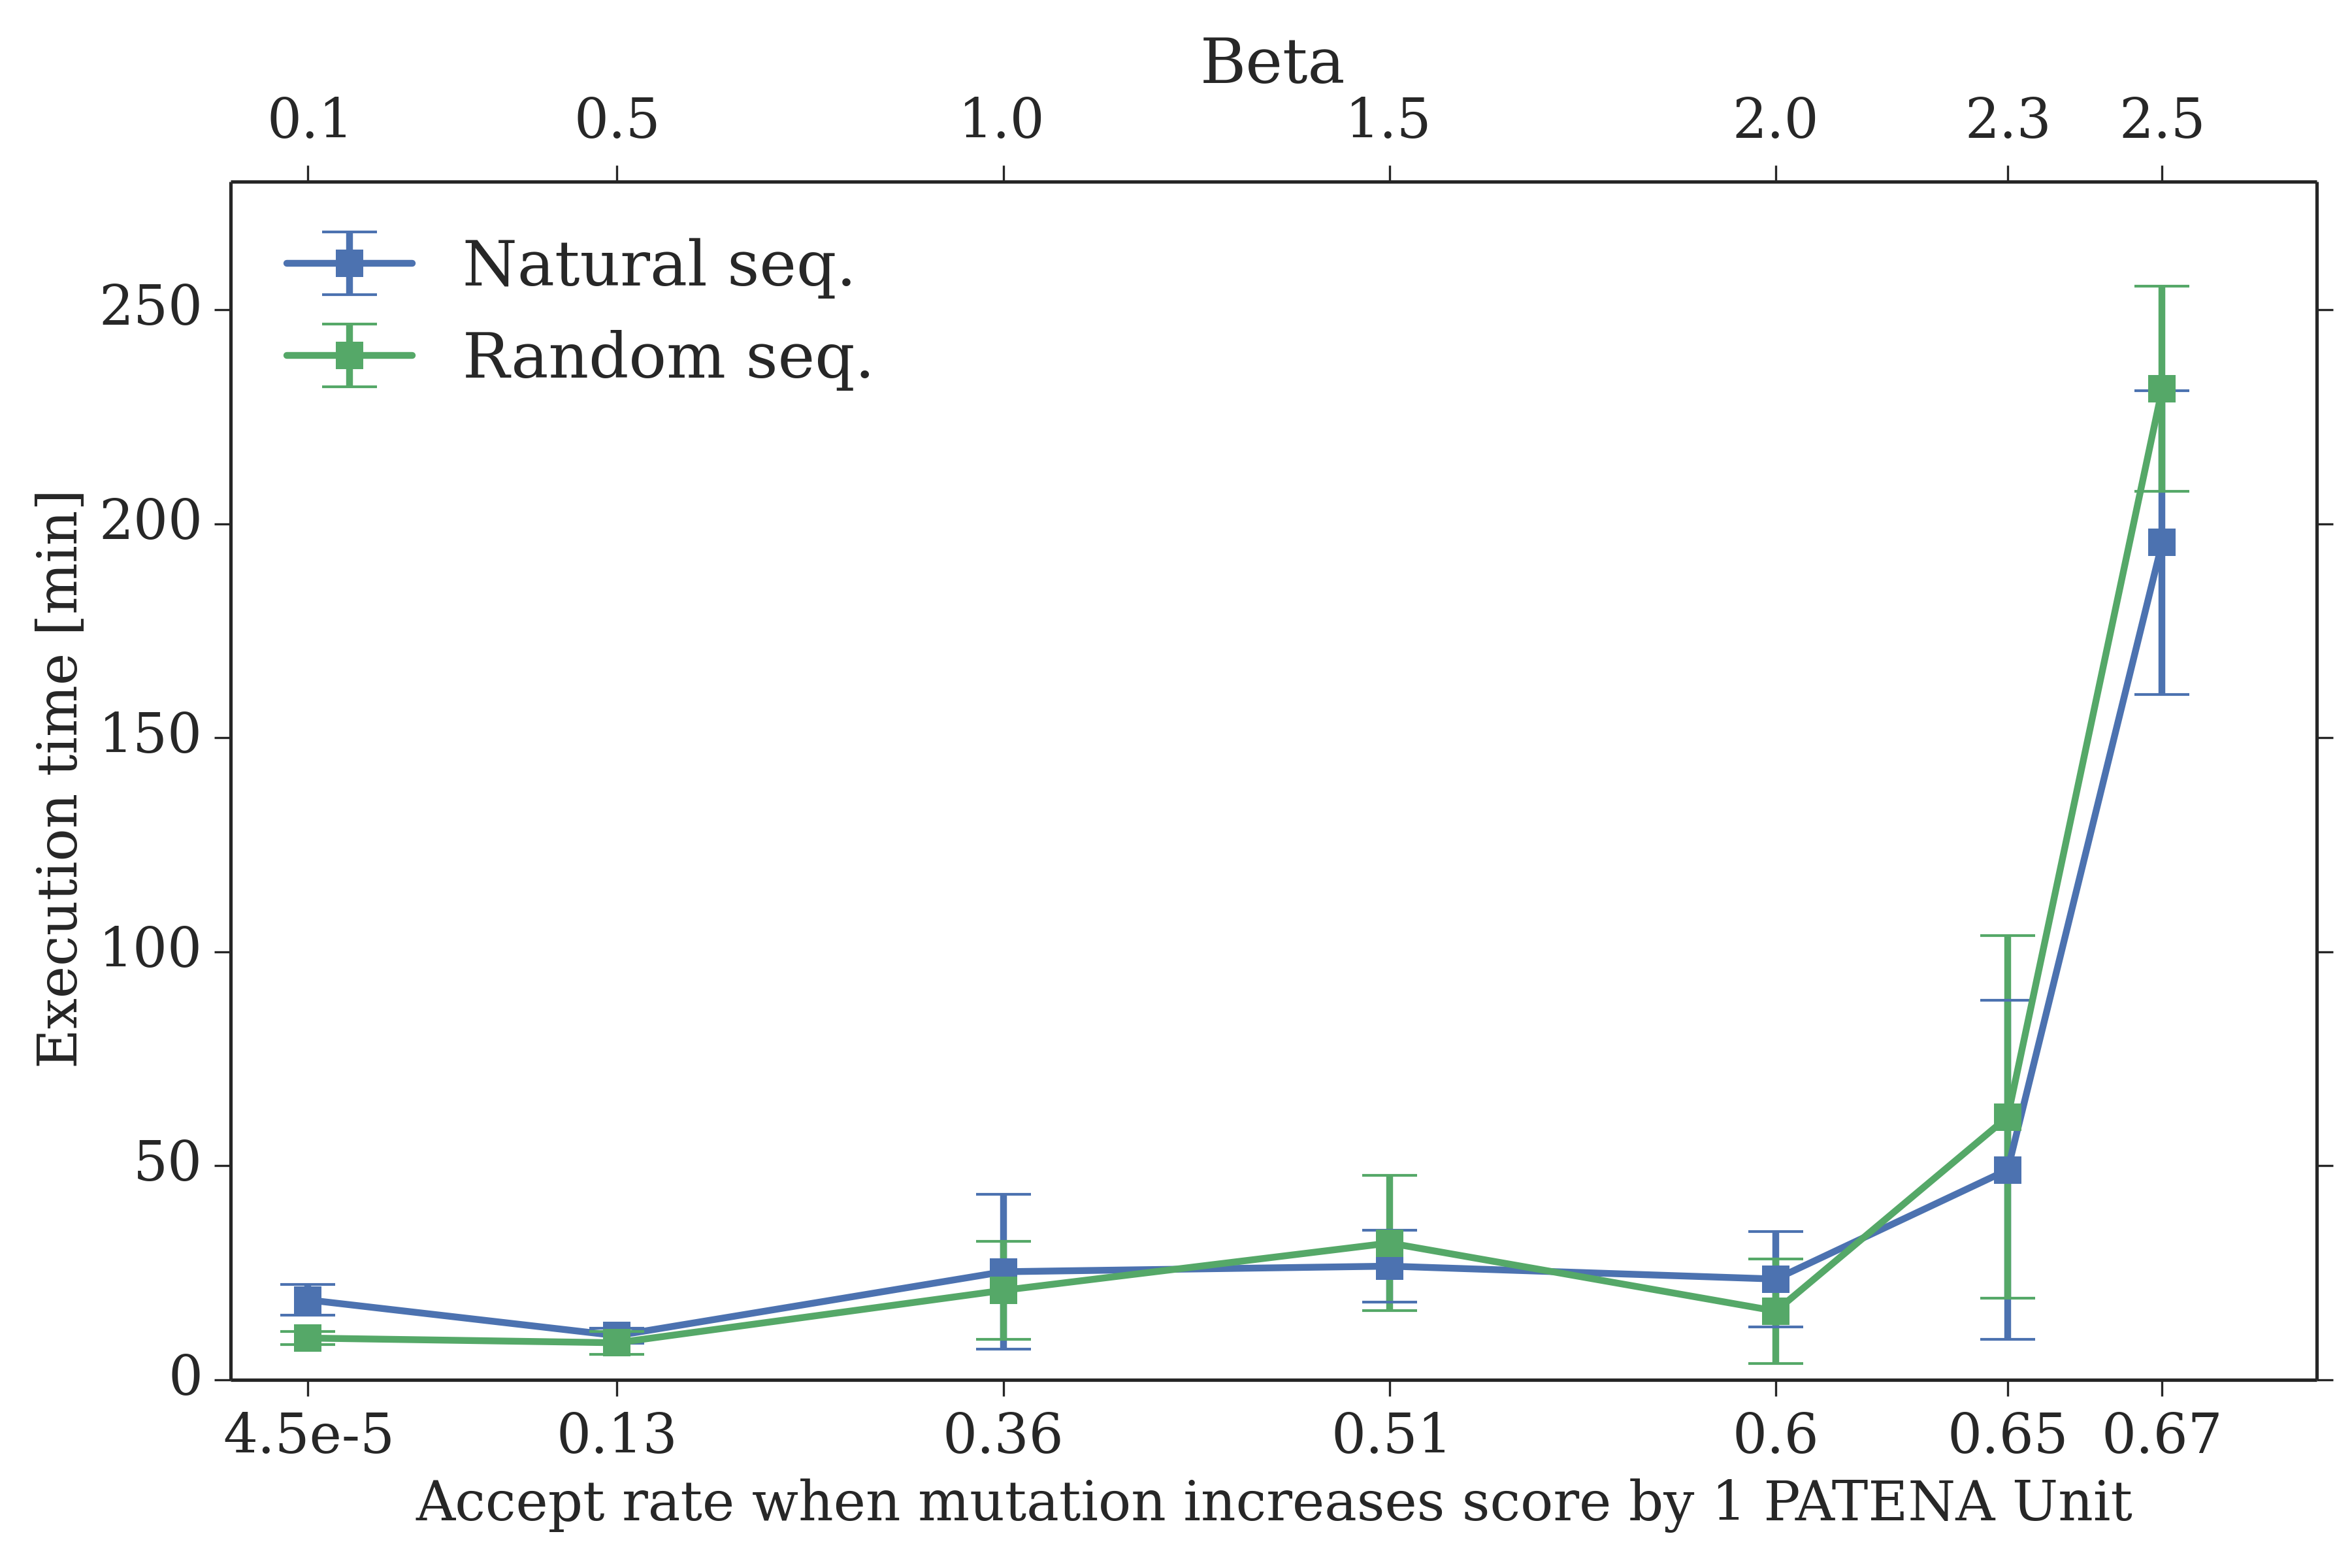
\includegraphics[width=330px,height=210px]{../img/beta-vs-time-length50-300dpi.png} 
\end{adjustwidth}
\end{frame}
















% we know it works and we have one effective value for beta.
% In this case, the execution profile is something like this.
% this graphic is only to get a better idea of how the execution profile looks like.
% how many mutations are required? in this particular execution we have a bit more than two hundred mutations 
% This number will be variable, since the method has some heuristics behind so it is not deterministic and it of course depends in the initial sequence and the length if it...
% that is an important aspect, what happens if we variate the length of the sequence??.....ACA ENGANCHO CON EL PROX. SLIDE
% 
% ***************************************************************
%      SCORE vs MUTACION  PARA 1 SOLA EJECUCION USANDO BETA=1.0
% ****************************************************************
\begin{frame}[plain]{Ejemplo de ejecución usando $\beta$ elegido (1.0)}
% Sample execution profile using defined $\beta$ (1.0)}
% \vspace{-0.5\baselineskip}
\begin{adjustwidth}{-1.5em}{-2.5em}
\centering

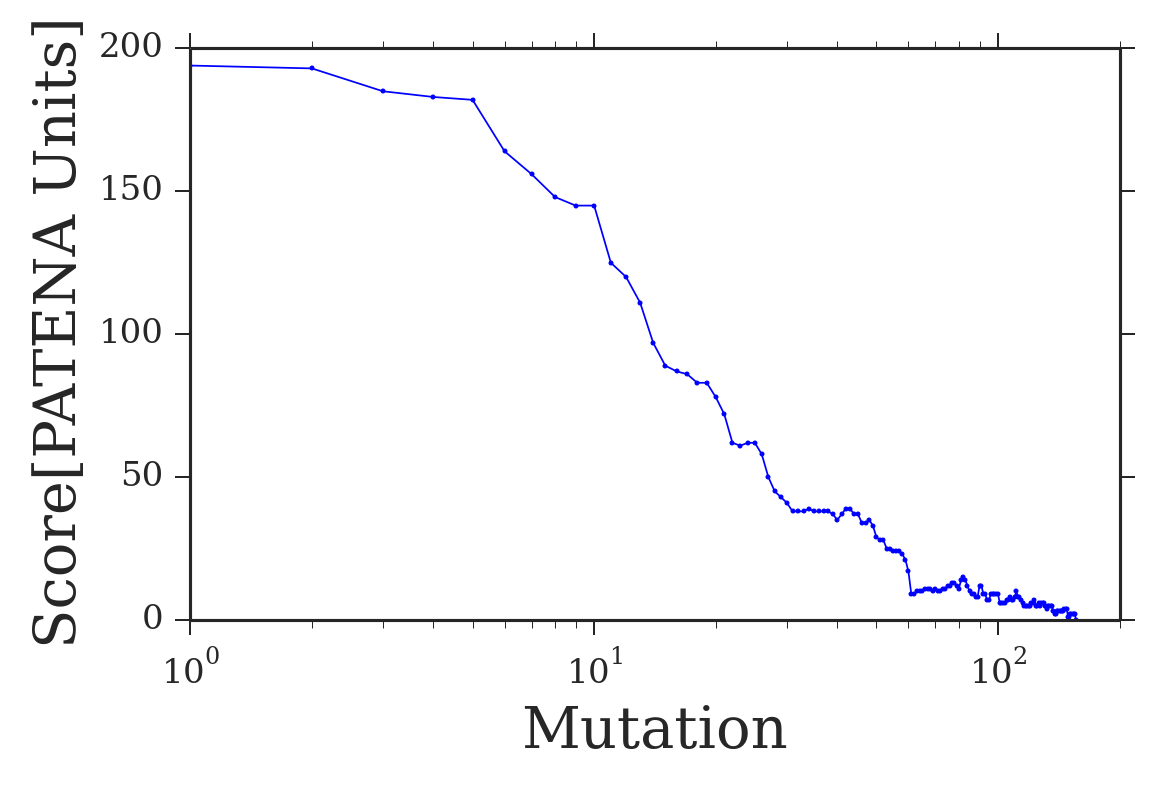
\includegraphics[width=330px,height=210px]{../img/iterationVsScore-individualBeta1-EXAMPLE.png}
% 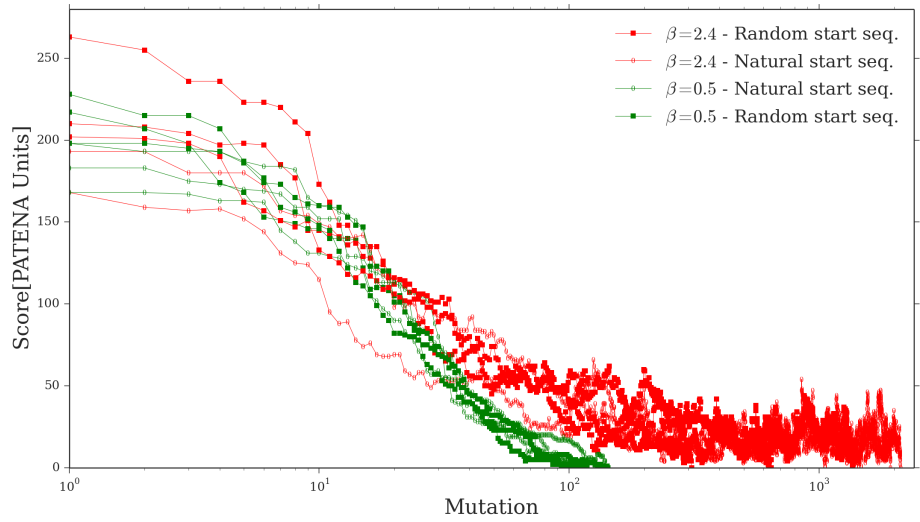
\includegraphics[width=330px,height=210px]{../img/scoreVsMutation-individual.png} 
\end{adjustwidth}
% \vspace{-\baselineskip}
\end{frame}








% to evaluate this we made a total of 36 different executions, starting from natural and random sequences of diffferent lengths.
% 

% *********************************************
%      TIEMPO EJECUCION vs LENGTH SECUENCIA
% *********************************************
\begin{frame}[plain]{Dependencia aproximadamente lineal con la longitud}
% Approximate linear dependence with length}

\centering
% Optimal $\beta$ range  
% [Length = 30] - [Random (n=3) and Natural (n=3) seq. / each $\beta$] \\
\begin{adjustwidth}{-1.5em}{-2.5em}
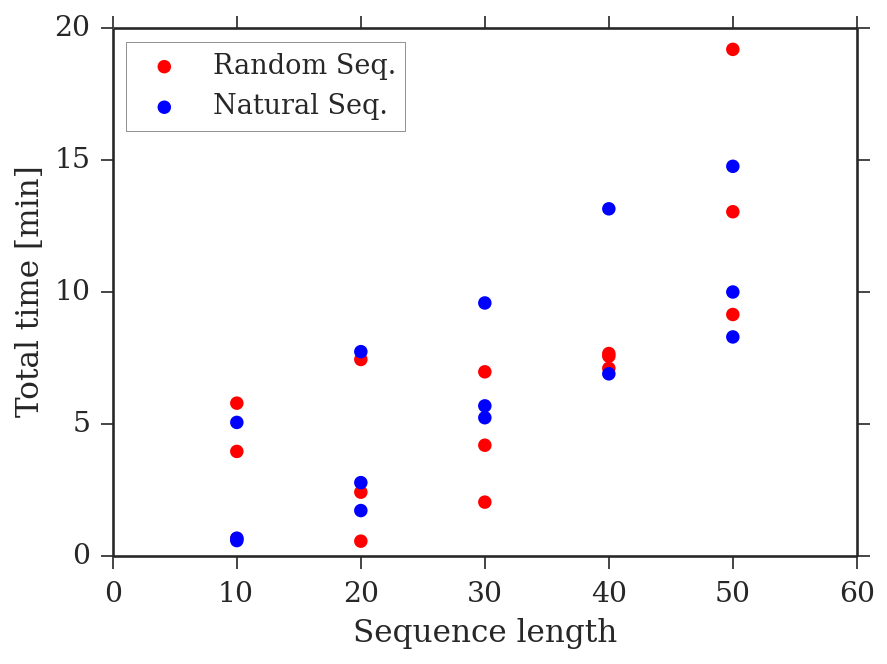
\includegraphics[width=330px,height=210px]{../img/lengthVsTime.png} 
\end{adjustwidth}
\end{frame}



















% ************************************************************
% AGREGAR UNA DIAP QUE ARRENQUE DICIENDO QUE YA TENEMOS E
% ARRANCAR DICIENDO QUE SABEMOS QUE EL MÉTODO FUNCIONA, PERO NO SABEMOS QUE TIPO DE RESULTADOS DEVUELVE
% EXPLICAR POR QUE USAMOS LA COMPOSICION ESTANDAR
% *******************************************************
% So, at the moment we have a method that allows to, at least, get some resulting designs.
% but i said first that one of the problems with linker design methods nowadays is that they may not provide de required diversity
% La diversidad resultante depende fuertemente de la composición que utilizamos para las mutaciones.
% 
% 
% La composicion estándar de Uniprot representa para la naturaleza una posibilidad de balancear, en la naturaleza, la diversidad requerida para armar un proteoma y la minimización del costo metabólico asociado a la secuencia.
% Entonces, ahora vamos a evaluar si utilizando esta composicion para las mutaciones en nuestro método, 
% podemos obtener resultados que sean suficientemente diversos pero que a la vez no representen un gran costo metabólico para la expresion.


\begin{frame}[plain]{Composición estándar}
% ANTES ACLARE COMO SE HACE PARA SELECCIONAR LA POSICION A MUTAR PERO NO SABEMOS COMO SELECCIONAMOS EL REEMPLAZO
% TODAVIA NO HABLE DE LA COMPOSICION QUE ESTAMOS USANDO PARA PROPONER LAS MUTACIONES
% ES DECIR, CUANDO SELECCIONAMOS UNA POSICION PARA CAMBIAR PORQUE EL MÉTODO LA SELECCIONA, NO ACLARE TODAVIA A QUE POSICION SE MUTA Y CON QUE FRECUENCIA
\begin{itemize}
 \item ¿Cómo seleccionamos el reemplazo para una mutación?
 \item ¿Cómo generamos secuencias random?
 \item Usamos composición extraída de UniProtKB
 \begin{itemize}
  \item No todos los aminoácidos tienen la misma frecuencia en la naturaleza
  \item Balance de diversidad y costo metabólico
%   BREVEMENTE.... en la naturaleza no todos  los aminoacidos se encuentran en la misma frecuencia...
% los organismos no solo minimizan el costo metabolico asociado a la biosintesis de proteínas (de esta forma, todas las proteínas esta)
% sino que tambien tienen que balancear esto con la diversidad de aminoacidos que se requiere para crear proteinas que puedan cumplir todas las funciones
  \end{itemize}
%   en nuestro caso tambien buscamos este balance ya que necesitamos cierta diversidad(para cummplir con distintos requerimientos impuestos) 
% y ademas, al estar disenando una secuencia que va a ser expresada queremos minimizar el costo metabolico
%  si nosotros imponemos esta composicion, es decir, tratamos que los diseños vayan hacia una composicion similar a la de uniprot podemos obtener un balance similar
 \item El diseño de linkers también requiere este balance. 
 \begin{itemize}
%  ya aplicamos esta composicion, ahora queda...
 \item Evaluar los diseños obtenidos por el método
 \end{itemize}

\end{itemize}

\end{frame}









% *********************************************
%      DIVERGENCIA: dividido en 2 slides
% *********************************************% 
% 
% 	DECIR SIEMPRE IDENTITY , PORQUE SI DIGO SIMILARITY SE CONFUNDE CON ALINEAMIENTO , ETC, ETC
% 		ACLARAR QUE COMO LOS RESULTADOS TIENEN LA MISMA LONGITUD, LA IDENTIDAD SE EVALUA SIMPLEMENTE COMPARANDO QUE POSICIONES TIENEN EXACTAMENTE EL MISMO RESIDUO
% 

% Here we have identity between a set of results(a total of 74 designs) obtained from running PATENA using the same initial sequence(these are the green bars).
% We have also blue bars indicating the identity that can be found between 1000 secuencias random al azar de largo=30 utilizando la composicion estandar
% Este background representa la maxima diversidad secuencial alcanzable con esta composici ́on.
% Conclusion: we can see, that, identity between resulting designs is greater than that between random sequences. Nevertheless the set of results is clearly heterogeneous.

% It is great to have such diversity but, if the user defines a sequence to start, the idea is to get a at least some similarity in the resulting design. 
% how similar are these results with the initial sequence??  ******** SWITCH DIAPO
\begin{frame}[plain]{{\small Algoritmo no determinístico: mismo input $\rightarrow$ diferentes resultados}}
% Nondeterministic algorithm: same input $\rightarrow$ different results}
\centering
\vspace{10px}
\begin{adjustwidth}{-2.5em}{-2.5em}
\begin{center}
\begin{adjustbox}{width=\textwidth}
Secuencia inicial única $\rightarrow$ 74 diseños - Identidad \textbf{entre secuencias resultantes}
\end{adjustbox}
\end{center} 
% \end{center}
% Fixed starting sequence $\rightarrow$ 74 designs - Identity \textbf{between final sequences}
% mayor que random pero claramente heterogeneas
\end{adjustwidth}
\hspace{10px} 
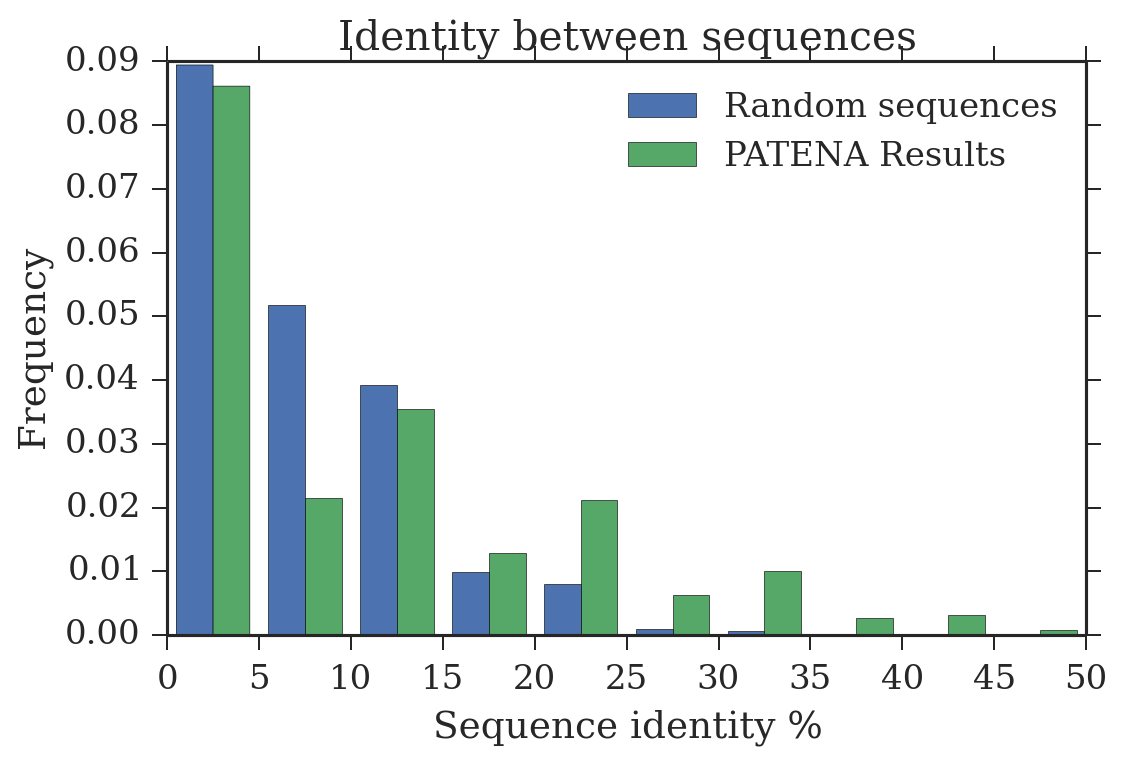
\includegraphics[width=275px,height=215px]{../img/againstAll-random.png}
% 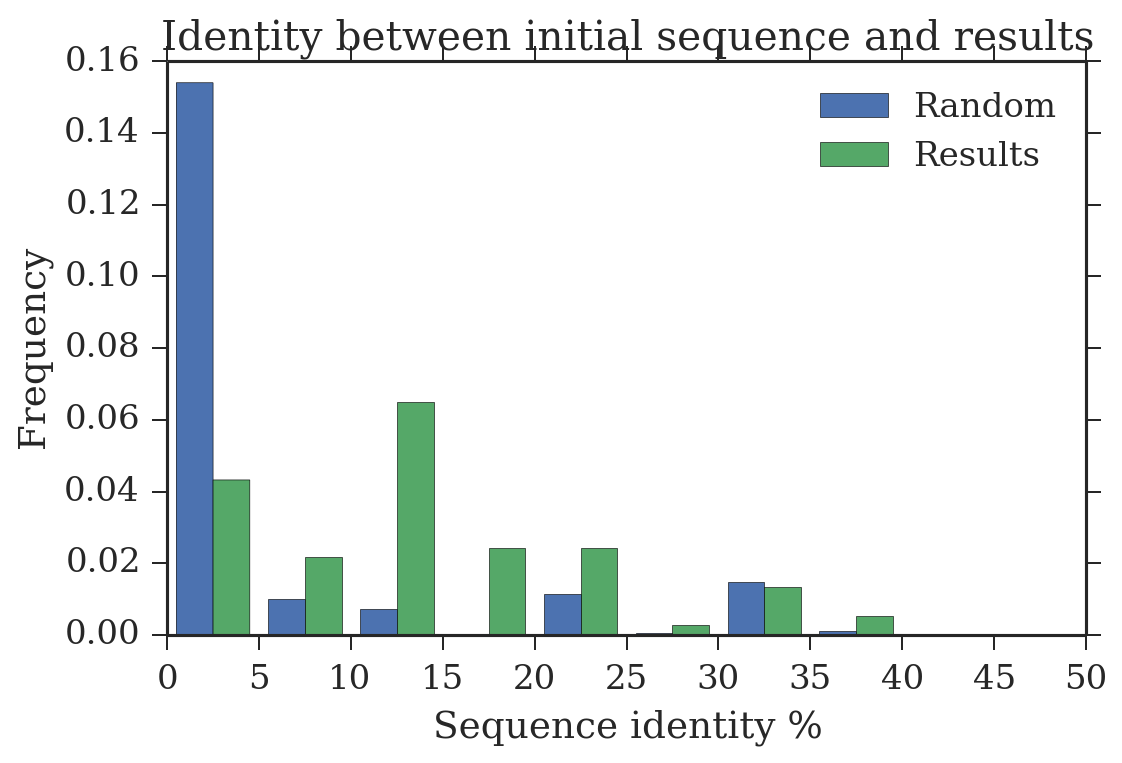
\includegraphics[width=175px,height=145px]{../img/againstInitial-random.png}
\end{frame}



% Using the same set of results we show here(in green bars) the identity between the set of results and the initial sequence.
% blue bars show the identity between that initial sequence and a set of random sequences of the same length
% Conclusion: the resulting set, although is quite diverse, still maintain certain similarity with initial sequence.
\begin{frame}[plain]{{\small Algoritmo no determinístico: mismo input $\rightarrow$ diferentes resultados}}
% Nondeterministic algorithm: same input $\rightarrow$ different results}
\centering
\vspace{10px}
\begin{adjustwidth}{-2.5em}{-2.5em}
% \hspace{10px}
\begin{center}
\begin{adjustbox}{width=\textwidth}
Secuencia inicial única $\rightarrow$ 74 diseños - Identidad \textbf{con la secuencia inicial}
% Fixed starting sequence $\rightarrow$ 74 designs - Identity \textbf{with initial sequence}
\end{adjustbox}
\end{center} 
% mayor que random pero claramente hubo bastantes mutaciones
\end{adjustwidth}
\hspace{10px}
% 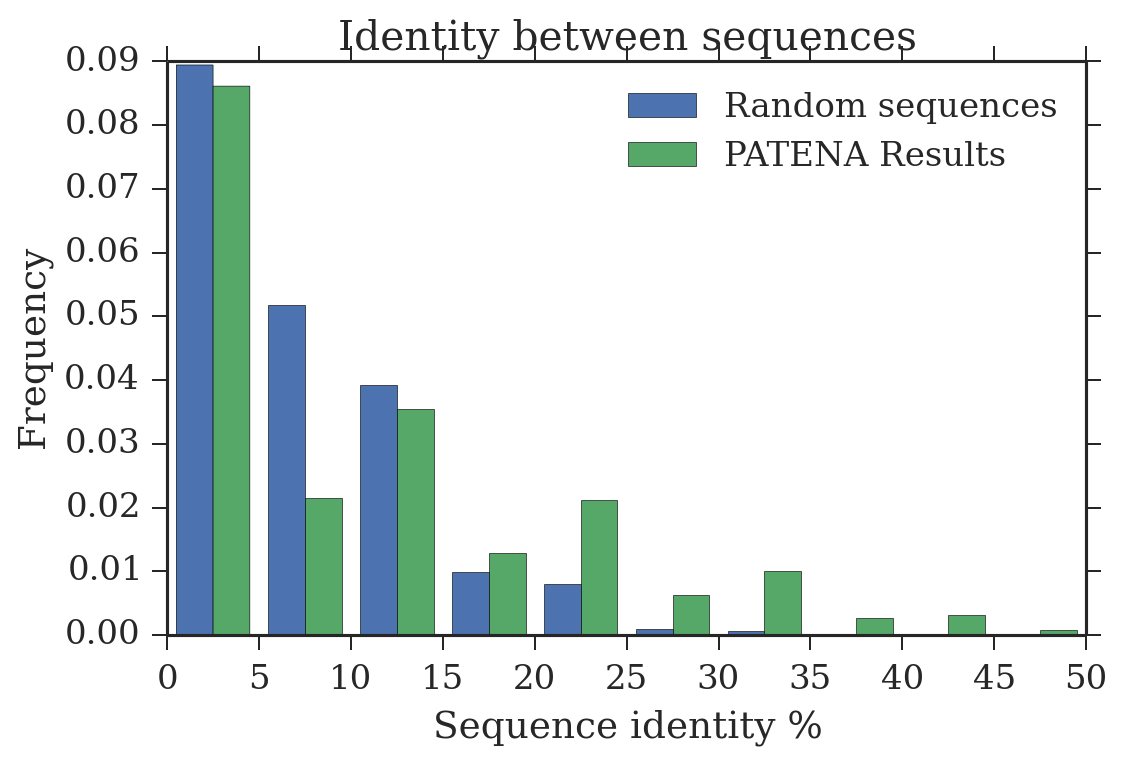
\includegraphics[width=175px,height=145px]{../img/againstAll-random.png}
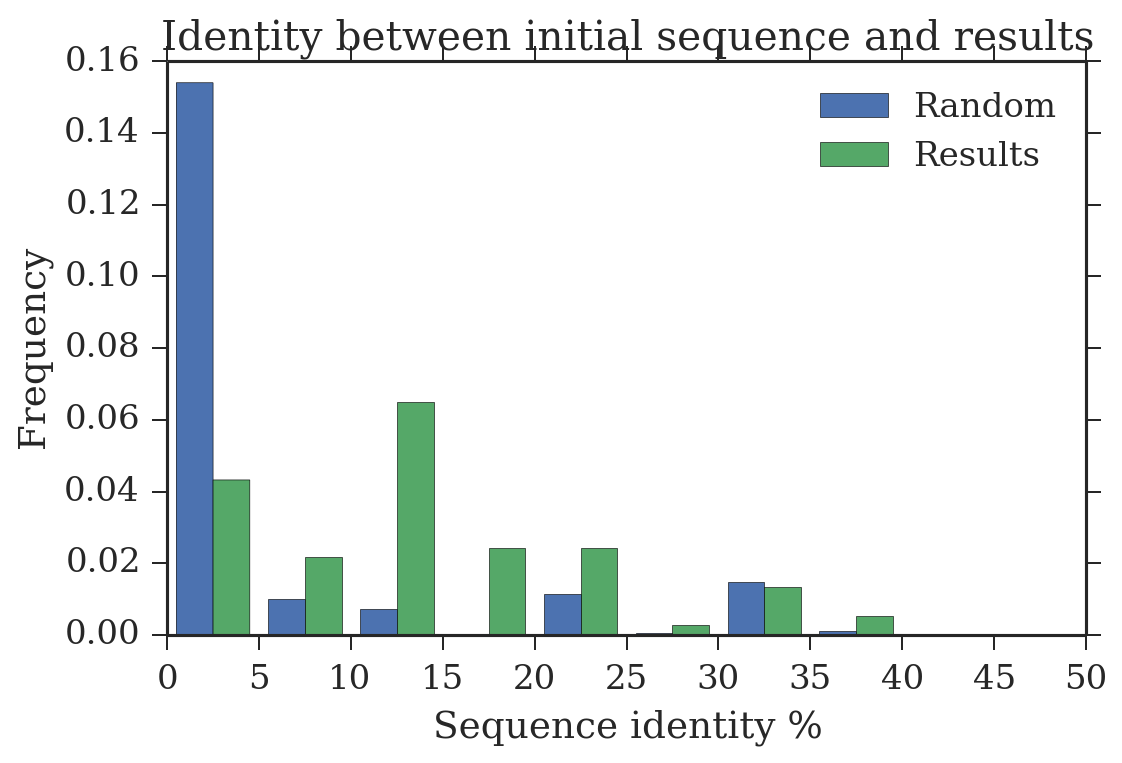
\includegraphics[width=275px,height=215px]{../img/againstInitial-random.png}
\end{frame}




















% *************************************************************
%  HASTA ACA YA SABEMOS QUE HAY CIERTA VARIEDAD EN LOS RESULTADOS, PERO DONDE ESTA UBICADA ESA DIVERSIDAD
%  LA IDEA DE USAR LA COMPOSICION ESTANDAR ERA OBTENER UN BALANCE DE ESTA CON EL MINIMO COSTO METABOLICO ASOCIADO
% *************************************************************

% INTENTAREMOS VER PRIMERO SI LA HETEROGENEIDAD SE LOCALIZA EN ALGUNA POSICION O TIENE ALGUN PATRON

\begin{frame}{Análisis de diversidad}
\centering
% {\large Secuencia inicial única $\rightarrow$ 74 diseños }
% \vspace{20px}
% Fixed starting sequence $\rightarrow$ 74 designs\\
\begin{adjustwidth}{-1.5em}{-2.5em}
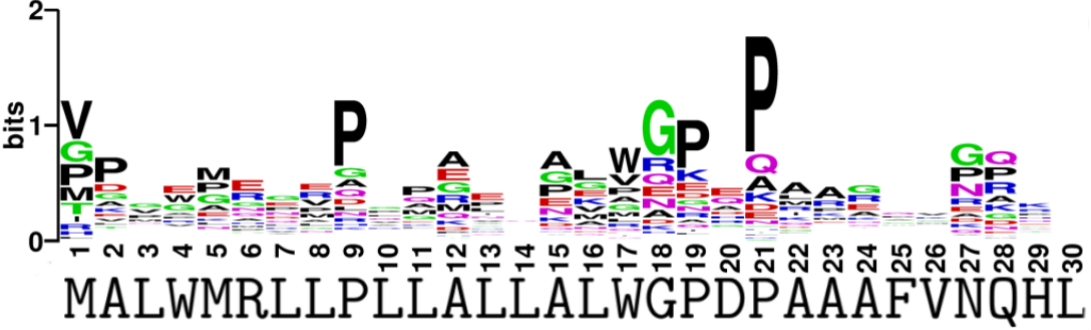
\includegraphics[width=340px,height=150px]{../img/logoInitial.png}\\ 
% \vspace{10px}
% \hspace{18px}
\includegraphics[width=325px,height=15px]{../img/sequence.png}
\end{adjustwidth}
\end{frame}








% ************************************************************* 
%    AGREGO EL LOGO DE LA SECUENCIA  ?????????????
% *************************************************************



% 
%      OBSERVED FREQUENCY vs EXPECTED FREQUENCY
\begin{frame}{Desviación de la composición estándar}
% {Standard composition deviation}
\centering
% Composición estándar
% Fixed starting sequence $\rightarrow$ 74 designs\\
% \begin{adjustwidth}{-1.5em}{-2.5em}
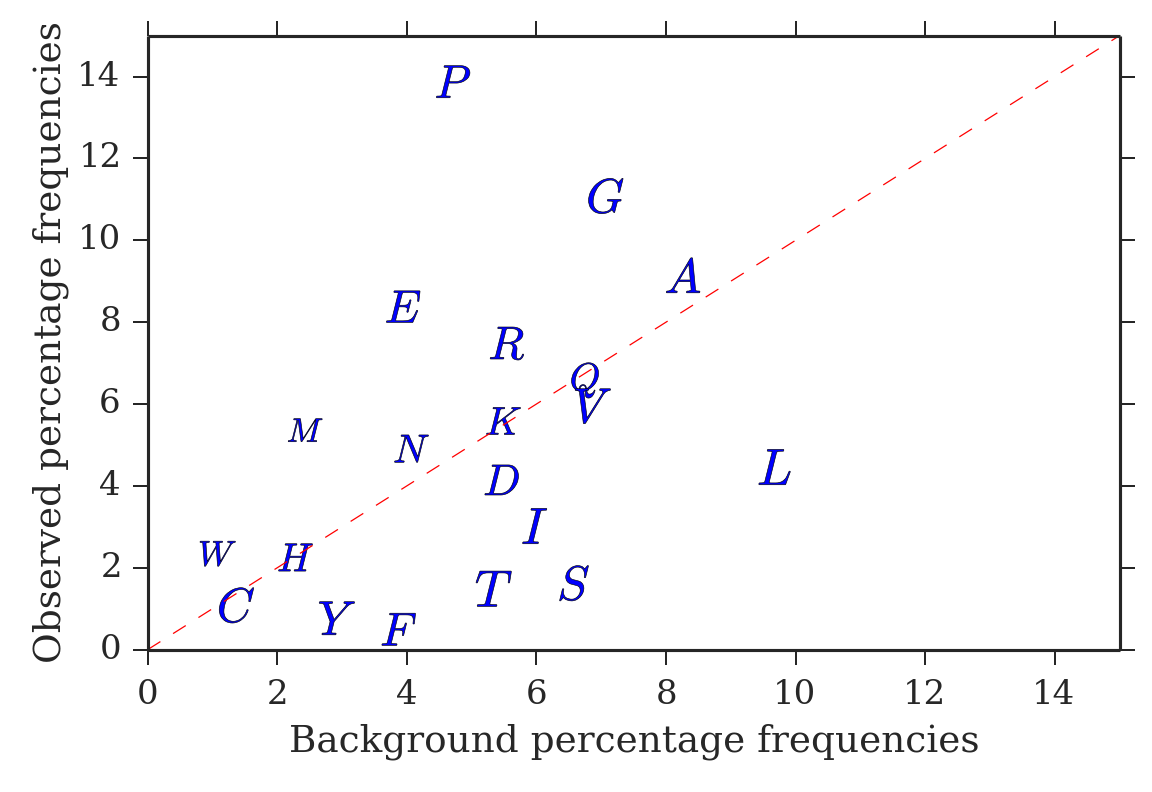
\includegraphics[width=310px,height=220px]{../img/frequenciesComparison.png}\\ 
% \end{adjustwidth}
\end{frame}







\begin{frame}{Aplicación completa}
% UNA VEZ EVALUADOS LOS DIFERENTES ASPECTOS TENEMOS UNA APLICACION COMPLETA PARA UTILIZAR QUE HASTA TIENE NOMBRE, SE LLAMA PATENA, PERO BUENO ESA ES UNA PEQUEÑA HISTORIA APARTE
% 
\begin{itemize}
 \item Disponible para utilizar bajo el nombre de PATENA
 \begin{itemize}
	\item Parámetros estandarizados: set de evaluación, beta, composición. 
	\item Modificación de parámetros para distintas ejecuciones %Aca deberia aclarar que al modificar 
  \end{itemize}
 \item Se agrega:
 \begin{itemize}
   \item Posibilidad de describir secuencias flanqueantes. 
   \item Posibilidad de definir la carga neta deseada.
   \item Posibilidad de obtener secuencias silentes en UV.
 \end{itemize}
 \item Primer paso para el desarrollo de un servidor 
%  Allows for development of server to design linker sequences.
\end{itemize}

 
\end{frame}























% To sum everything up
% PATENA can find suitable linkers in a short execution time, that is, in the order of tens of minutes usually
% We can also obtain a set of designs showing high diversity, which is ideal since we can fill lot of different preferences.
% The input can be very simple so this method allows to develop a server to easily obtain linker designs. 
\begin{frame}{Conclusión}
\begin{itemize}
  \item El método permite obtener secuencias linker en un tiempo de minutos.
  \item Los diseños resultantes son diversos en secuencia.
\end{itemize}
% estos dos resultados son compatibles con una de las hipotesis que planteamos cuando comenzamos este trabajo y no se
% 
\vspace{20px}

\textbf{Resultados compatibles con la hipótesis inicial de que existe un gran número de secuencias con las características que definimos como deseables para un linker}
%  \item PATENA can find suitable protein linkers in a short execution time.
%  \item The set of designs that can be obtained from the same sequence shows high diversity. 
%  \item We interpret that the space of suitable linker sequences is a large fraction of the whole sequence space.
\end{frame}



\begin{frame}
\begin{center}
 \huge Gracias
\end{center}
\end{frame}


























% *************************************************************
% *************************************************************
% *************************************************************
% 			EXTRA
% *************************************************************
% *************************************************************
% *************************************************************







% *************************************************************
% 		SEQUENCE LOGO  
% *************************************************************


% 
% \begin{frame}
% \begin{adjustwidth}{-1.5em}{-2.5em}
% 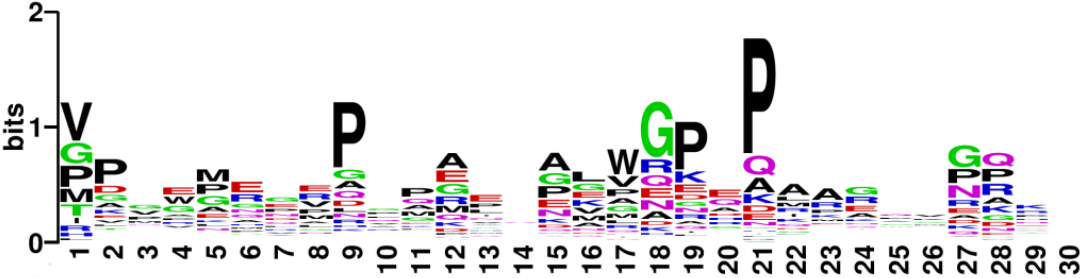
\includegraphics[width=340px,height=150px]{../img/logo.png}\\ 
% % \vspace{10px}
% \hspace{18px}
\includegraphics[width=325px,height=25px]{../img/sequence2.png}
% \end{adjustwidth}
% \end{frame}
% 
% 
% 
% 









% *************************************************************
%     ITERATION vs SCORE(MEAN)
% *************************************************************
\begin{frame}
\begin{adjustwidth}{-2.0em}{-2.0em}
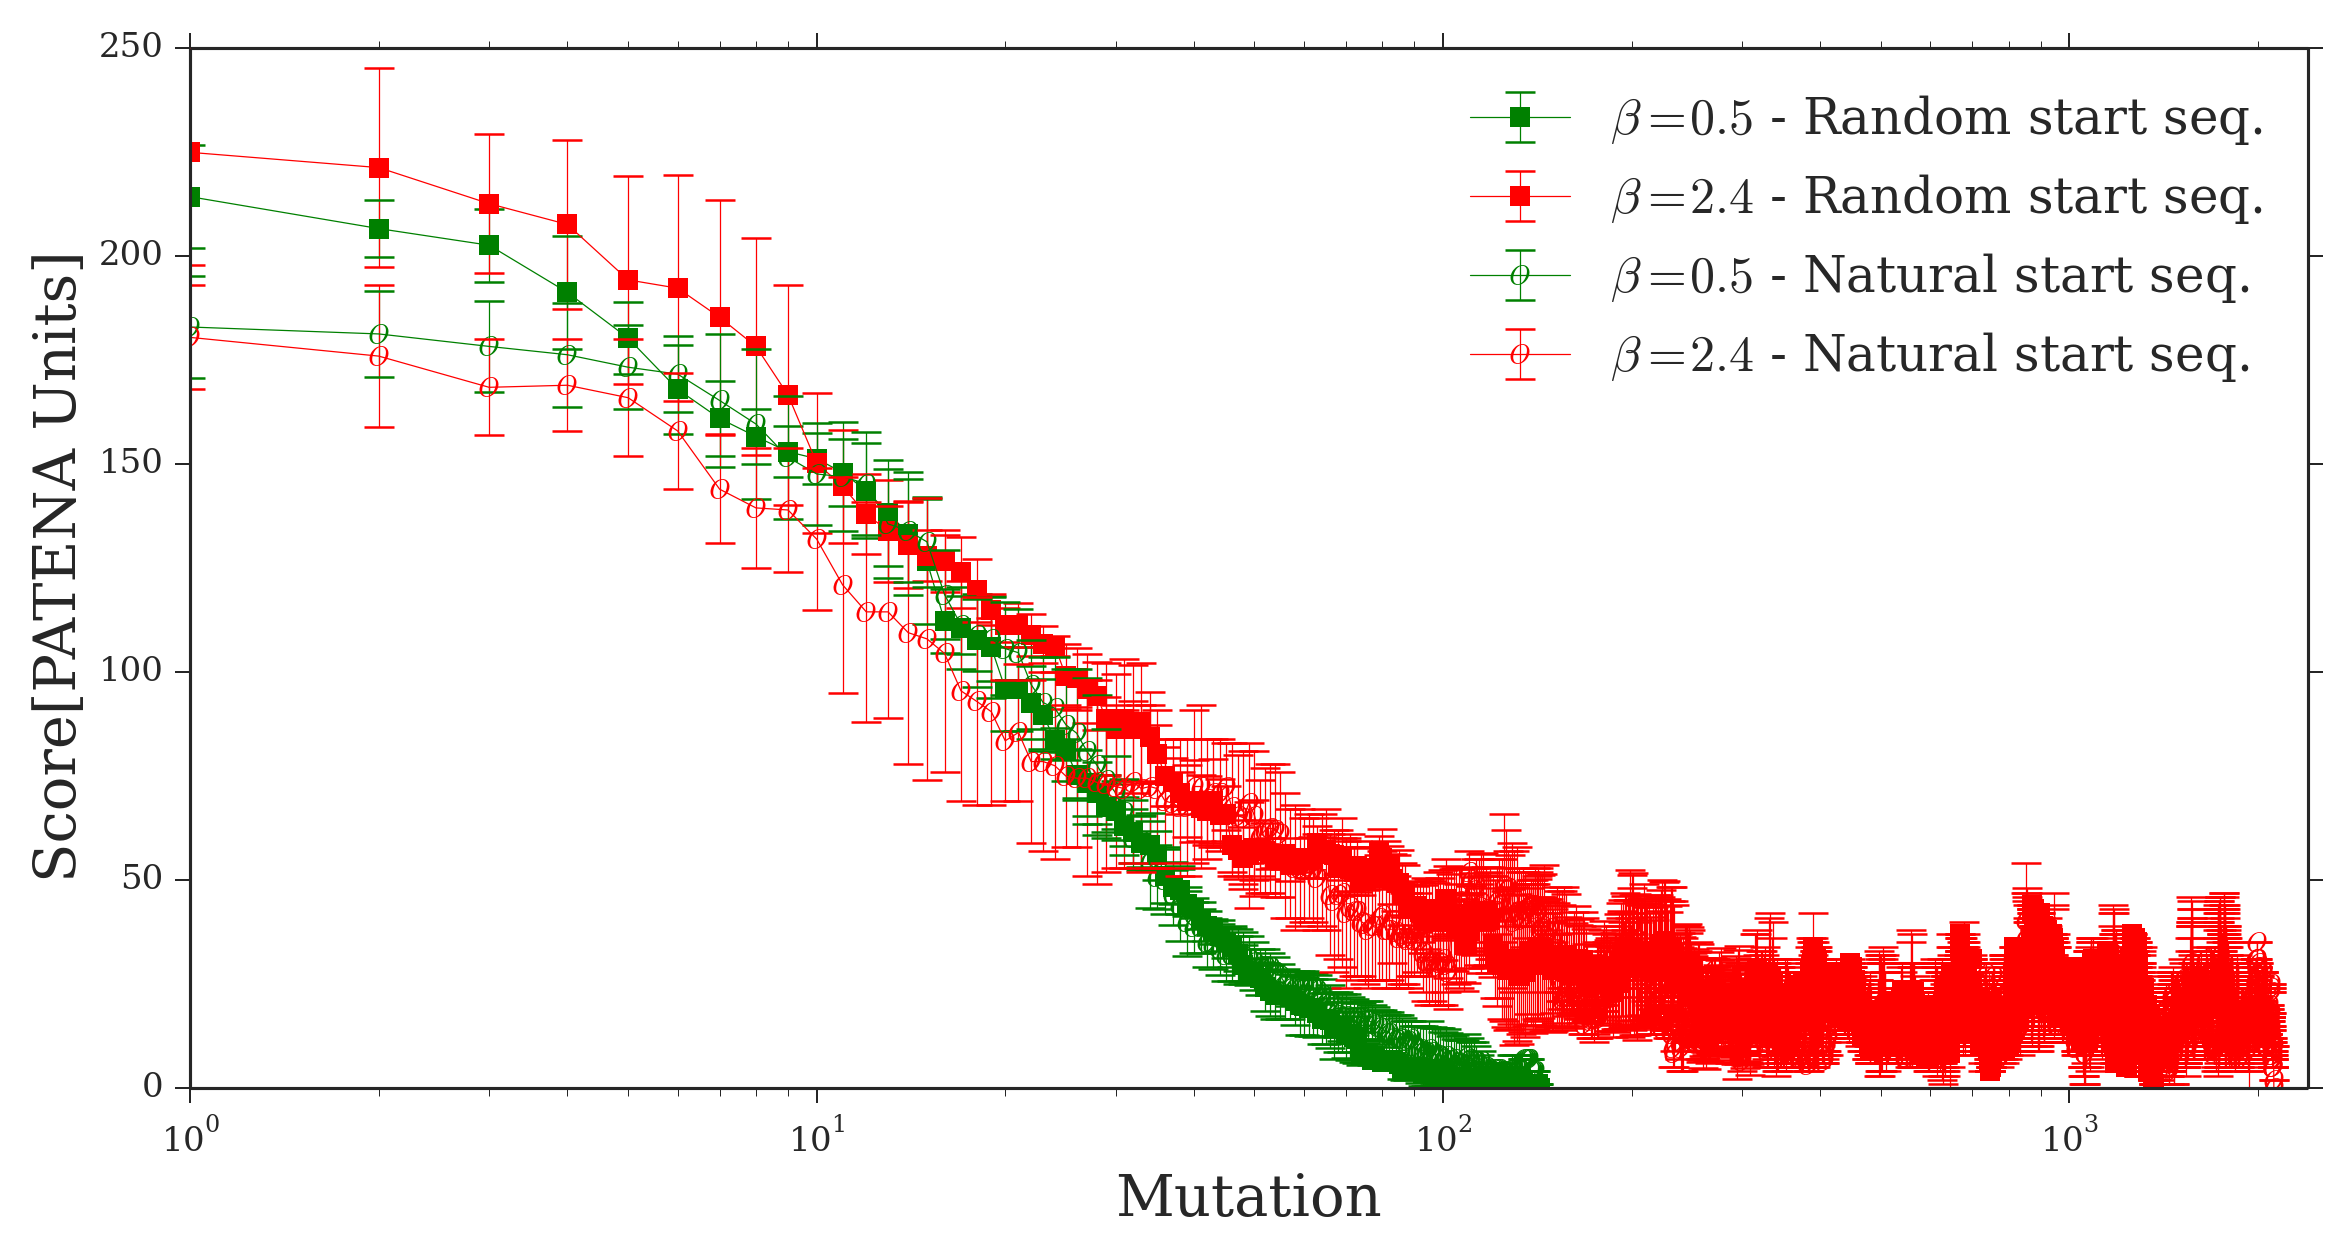
\includegraphics[width=340px,height=250px]{../img/iterationVsScore-mean.png} 
\end{adjustwidth}
\end{frame}




% *************************************************************
%     ITERATION vs MUT. ATTEMPTS(MEAN)
% *************************************************************
\begin{frame}
\begin{adjustwidth}{-2.0em}{-2.0em}
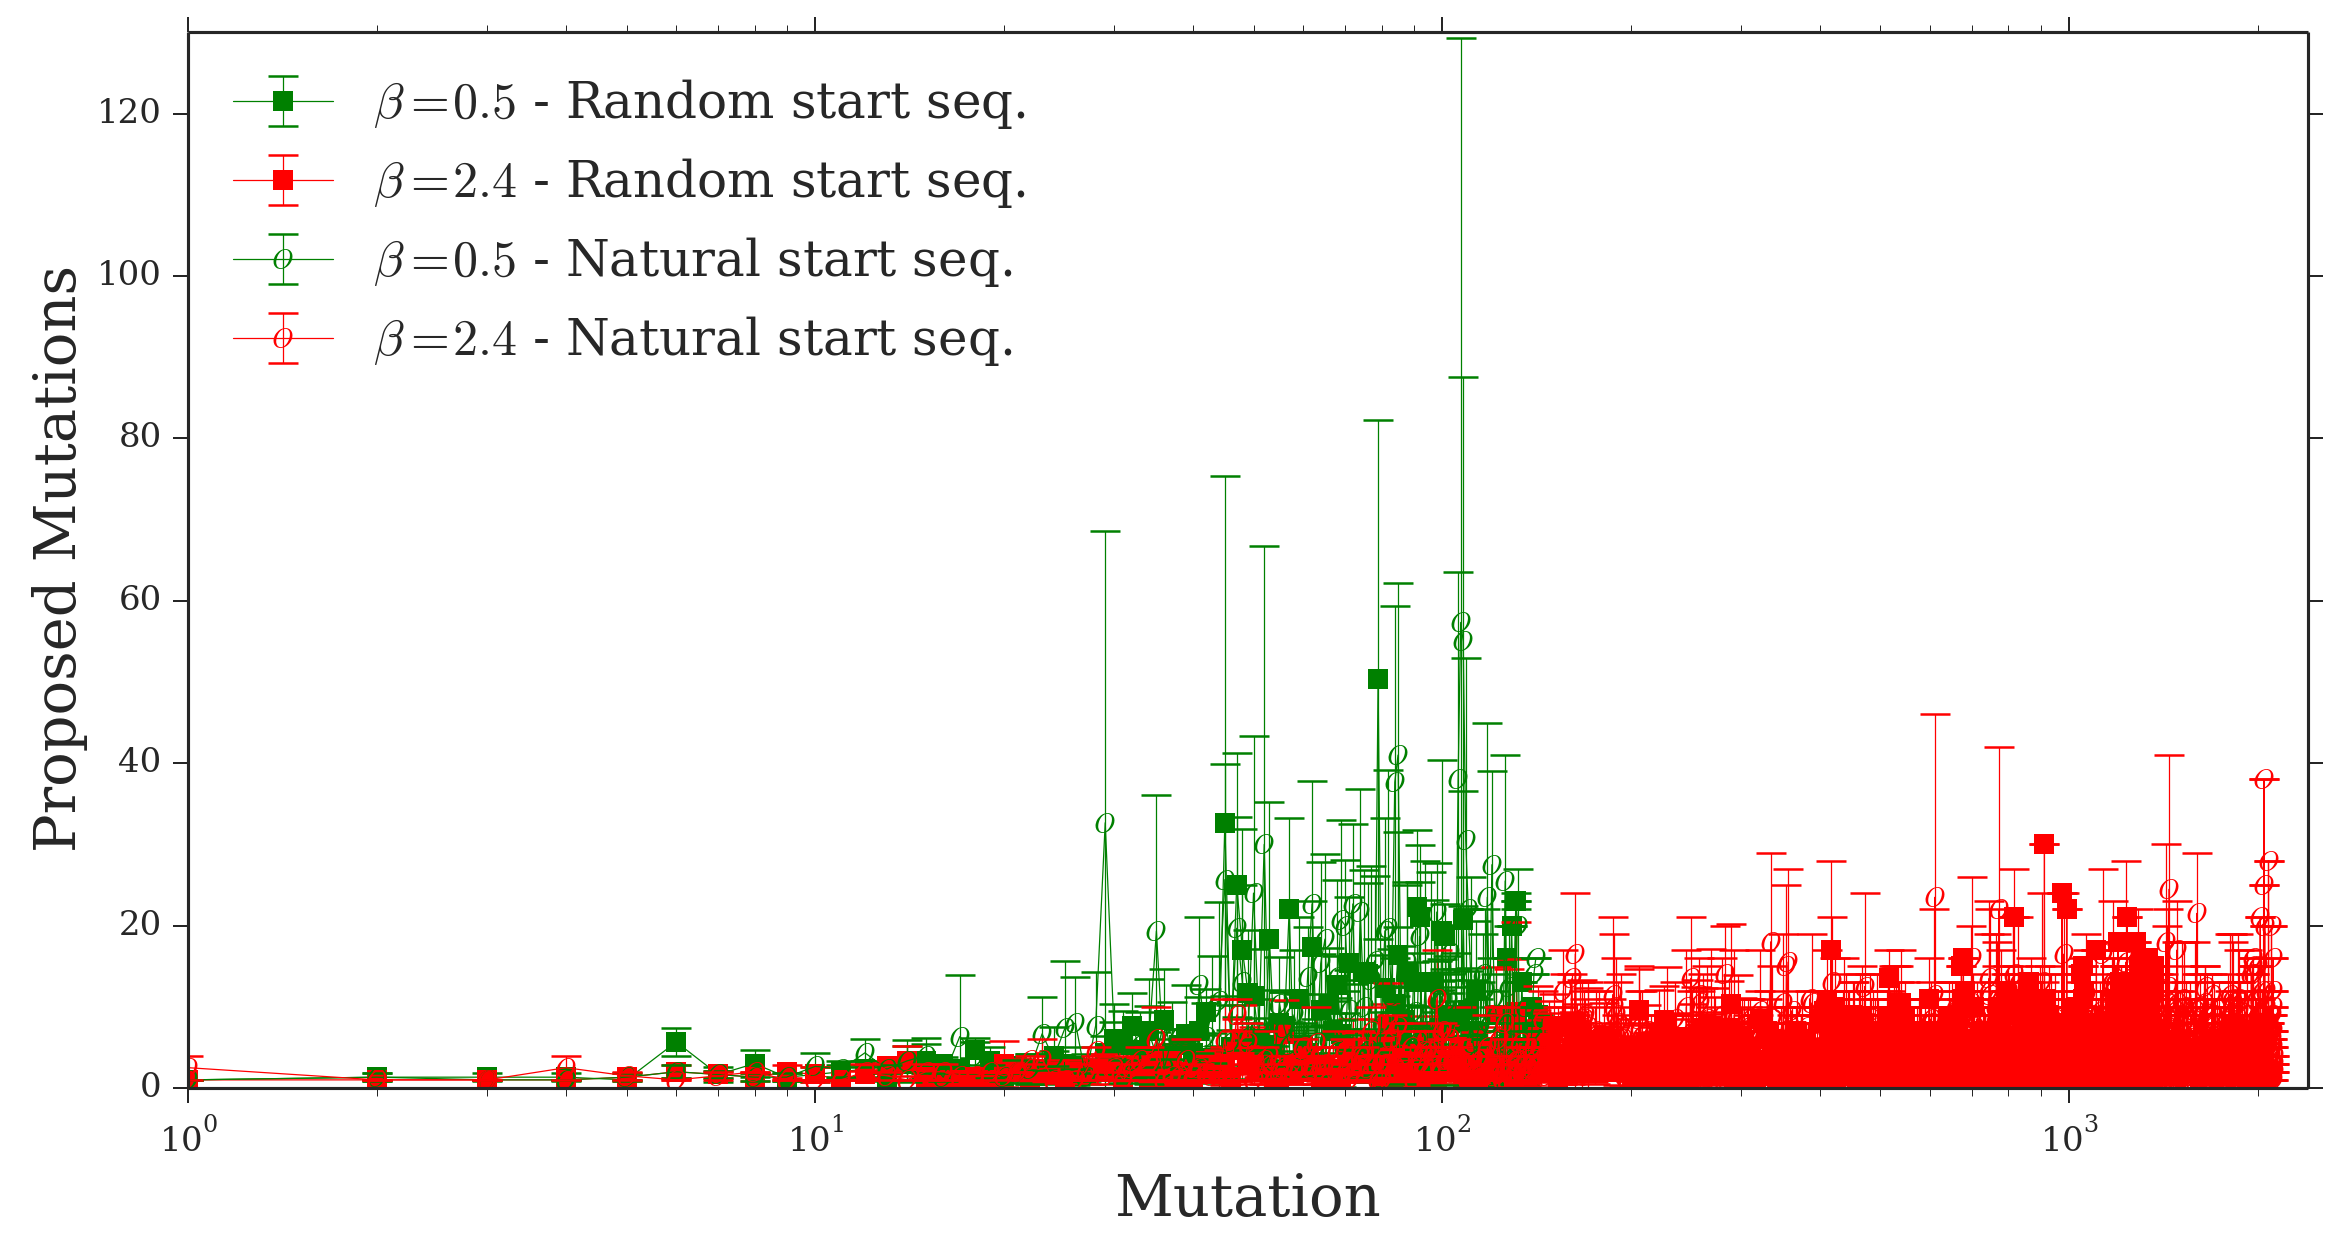
\includegraphics[width=340px,height=250px]{../img/iterationVsMutAttempts-mean.png} 
\end{adjustwidth}
\end{frame}



% *************************************************************
% 		BETA  vs  MUT. ATTEMPTS + ITERATIONS
% *************************************************************
\begin{frame}
\begin{adjustwidth}{-1.5em}{-2.5em}
% 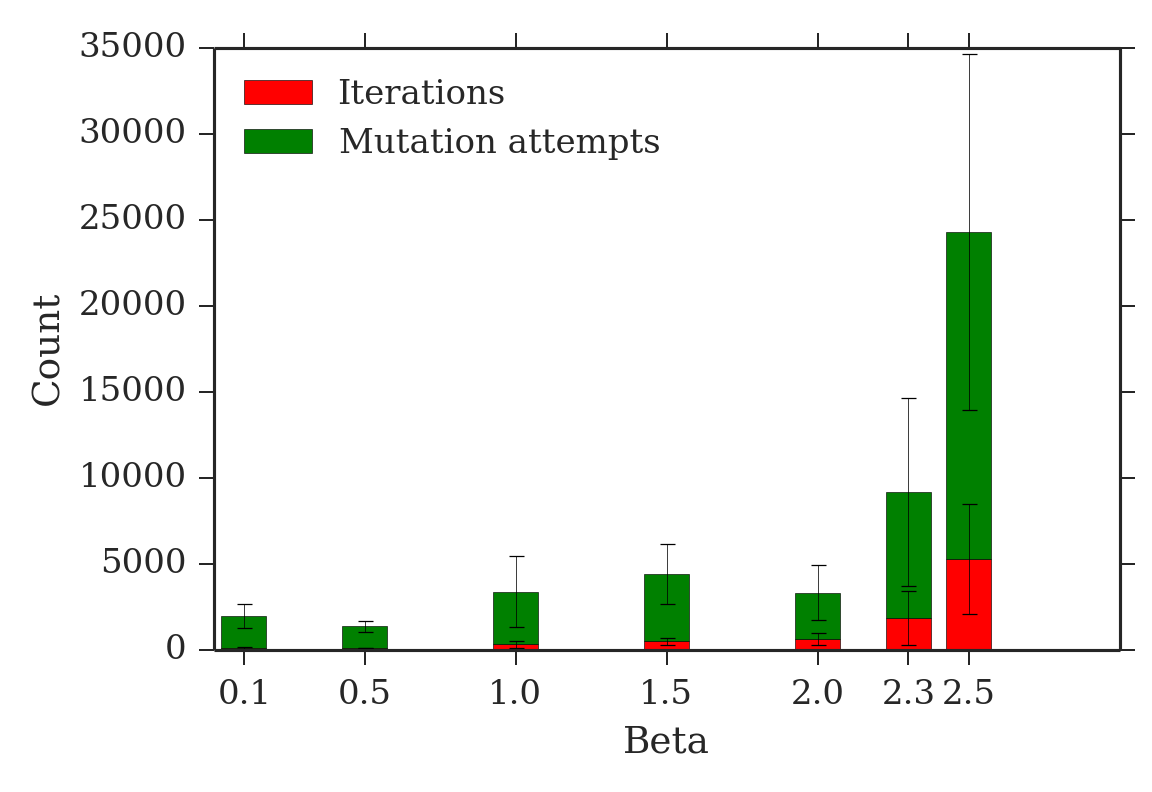
\includegraphics[width=340px,height=250px]{../img/betaVsIterations-MutAttempts.png}\\
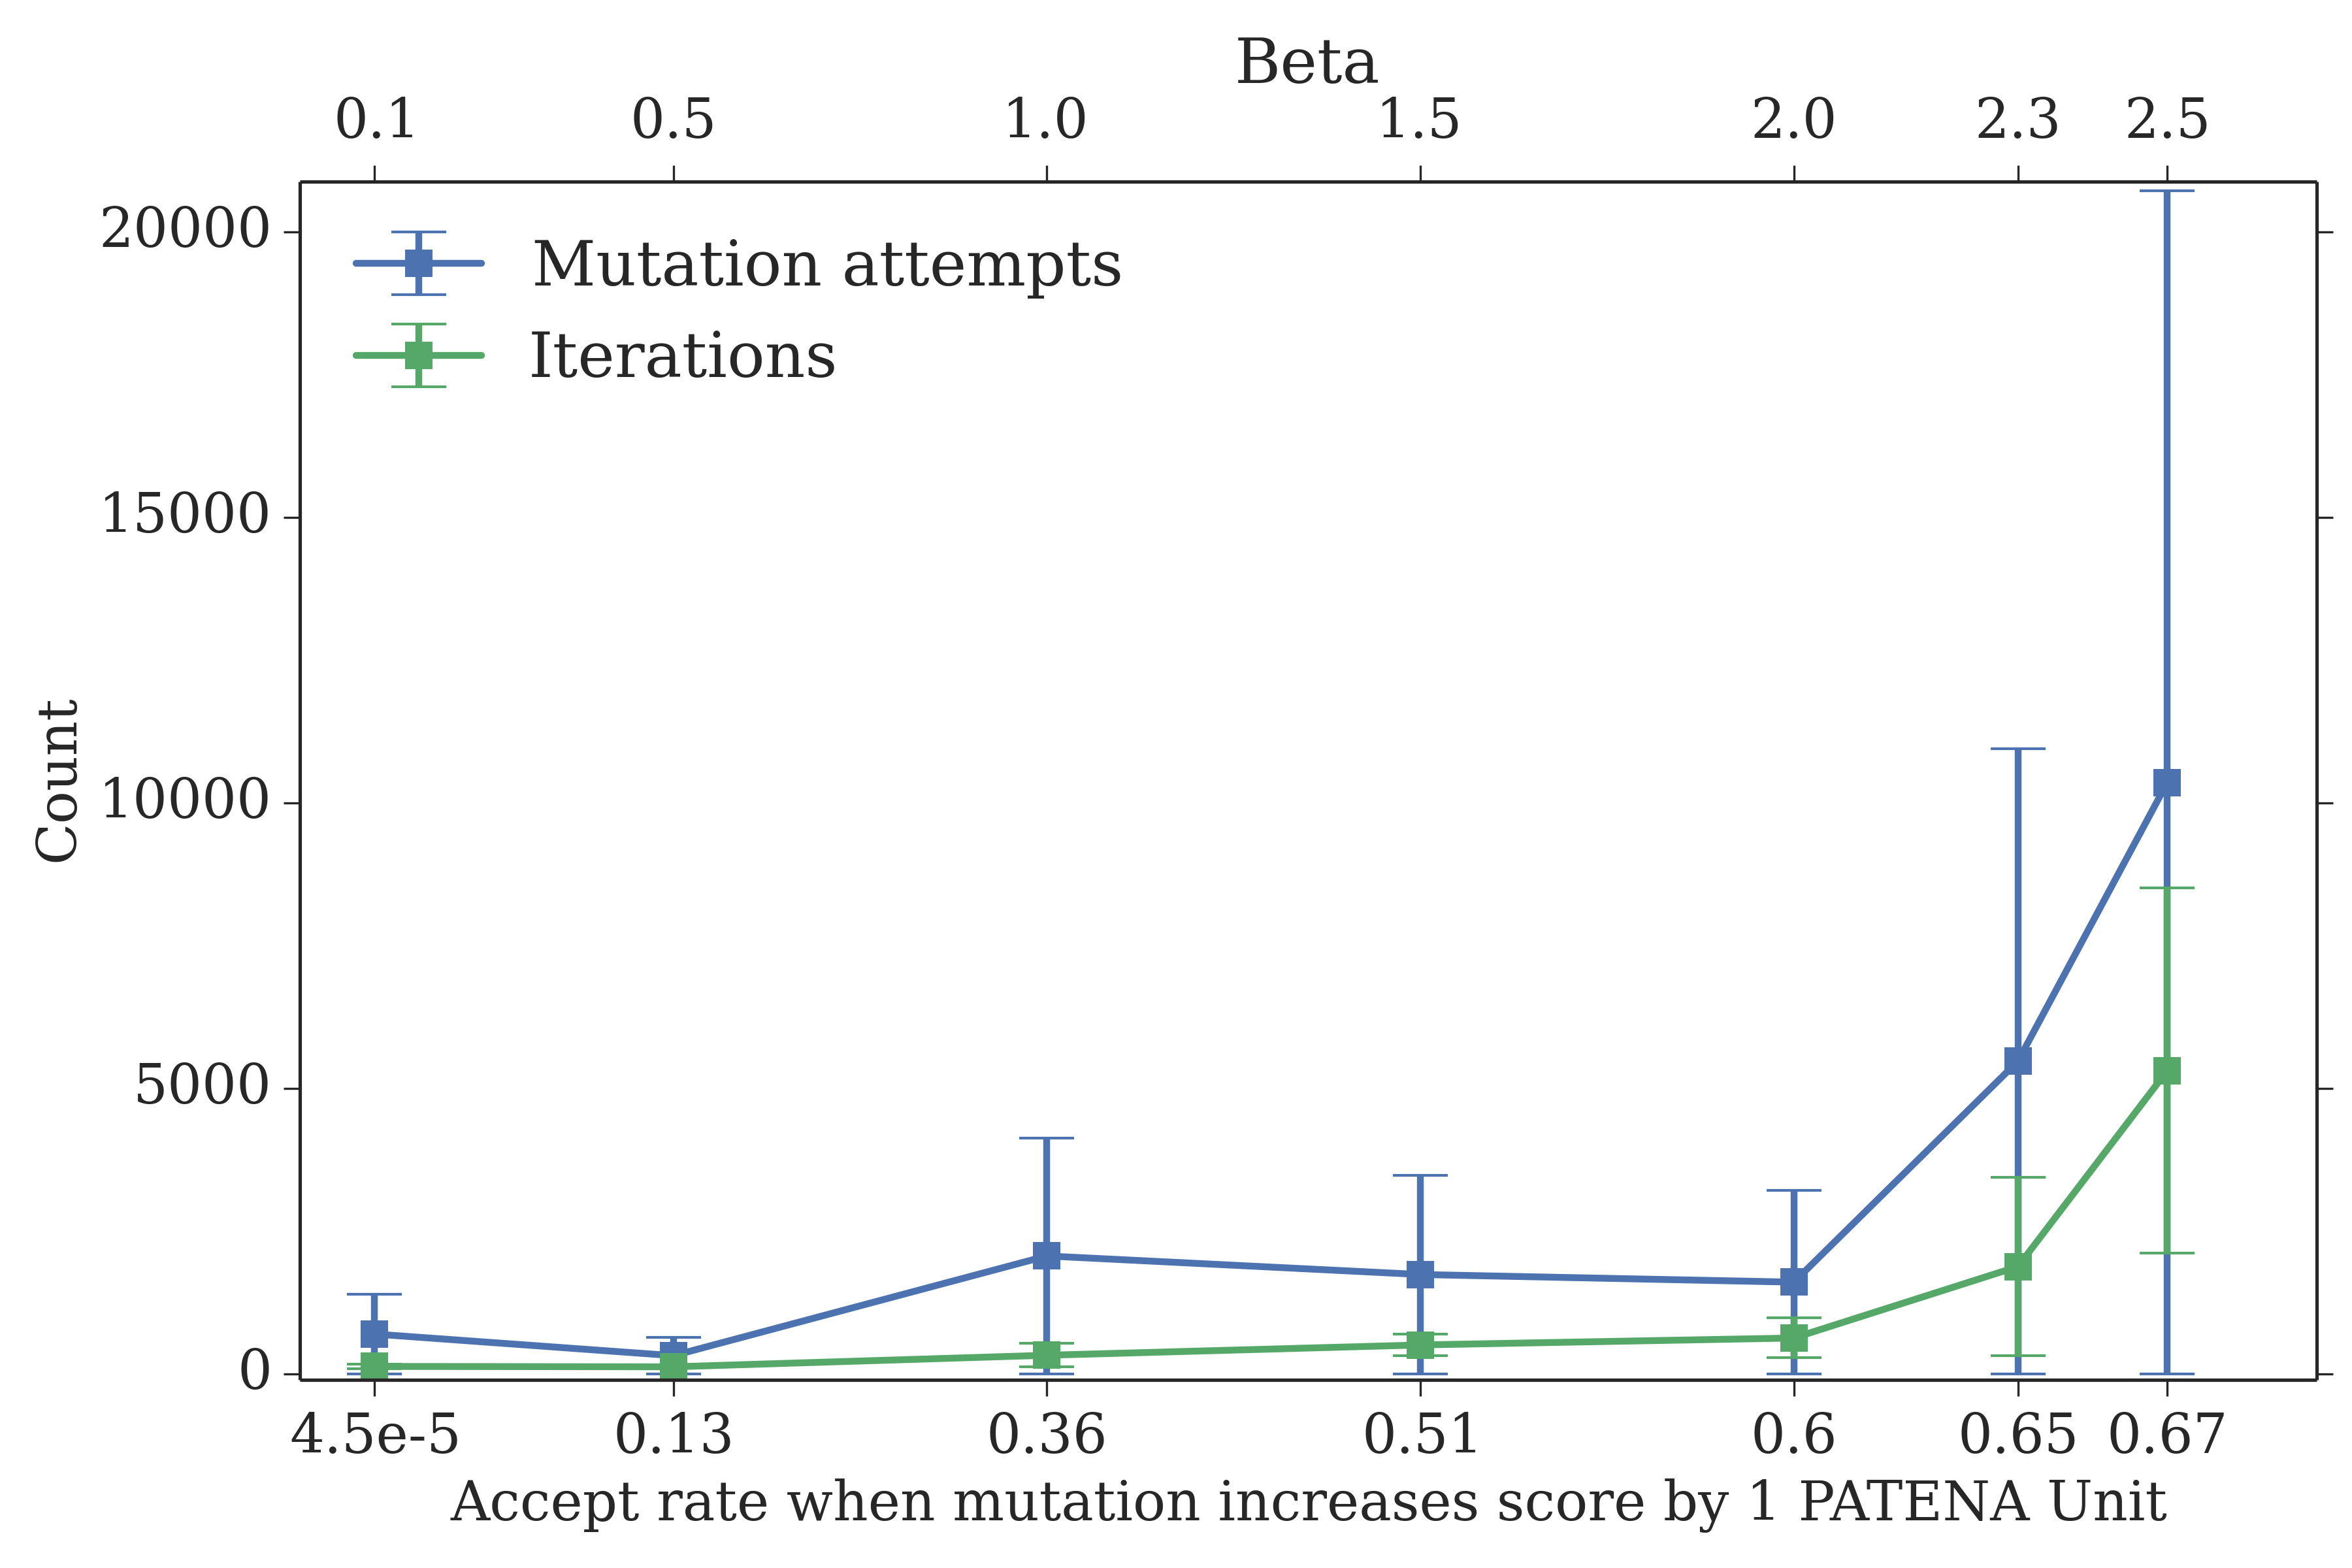
\includegraphics[width=340px,height=250px]{../img/beta-vs-Mut-iterations}\\
\end{adjustwidth}
\end{frame}








% 
% \begin{frame}
% \centering
% Fixed starting sequence $\rightarrow$ 74 designs \\
% \begin{adjustwidth}{-1.5em}{-2.5em}
% 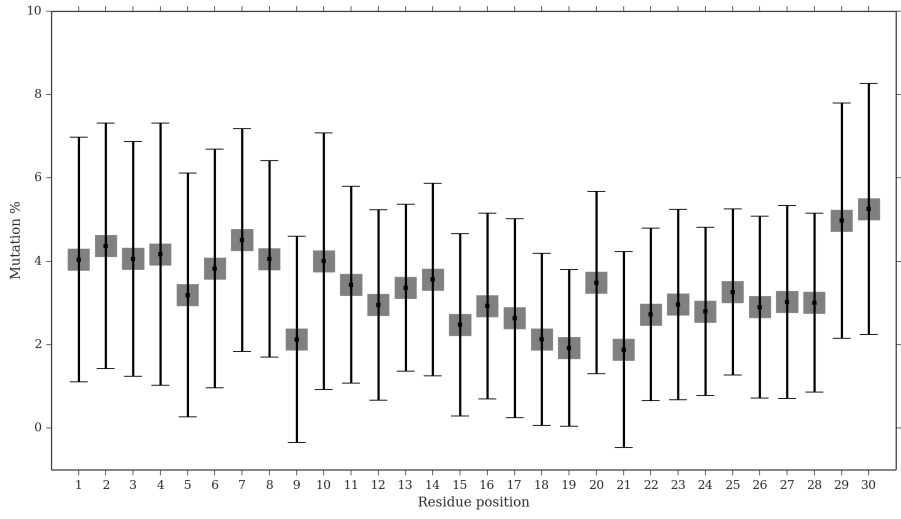
\includegraphics[width=340px,height=150px]{../img/mutationsPerPosition.png}\\ 
% % \vspace{10px}
% \hspace{25px}
\includegraphics[width=310px,height=10px]{../img/sequence.png}
% \end{adjustwidth}
% \end{frame}
% 





\begin{frame}
\centering
Fixed starting sequence $\rightarrow$ 74 designs - Beta 0.5 , 0.1\\

\begin{adjustwidth}{-1.5em}{-2.5em}
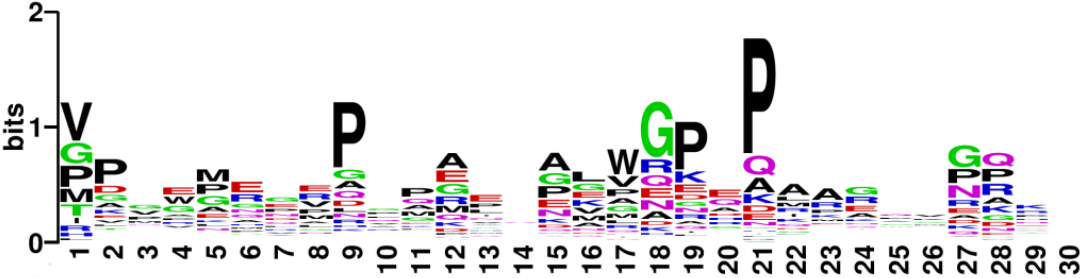
\includegraphics[width=340px,height=80px]{../img/logo.png}\\ 
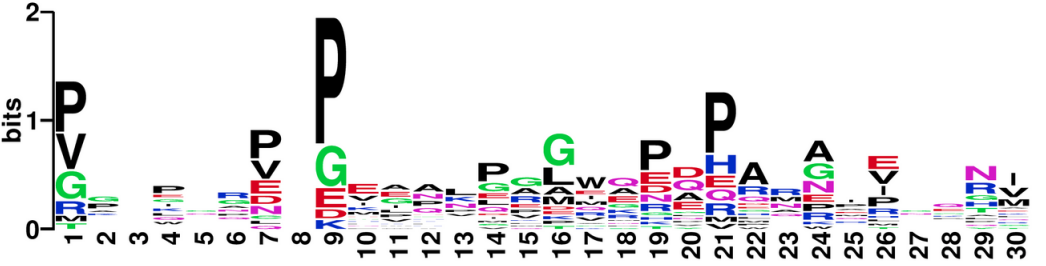
\includegraphics[width=345px,height=80px]{../img/logoBeta0-1.png}\\ 
\vspace{5px}
\hspace{18px}
\includegraphics[width=324px,height=15px]{../img/sequence.png}
\end{adjustwidth}
\end{frame}











% The name
\begin{frame}{Limpio como una patena}
\centering
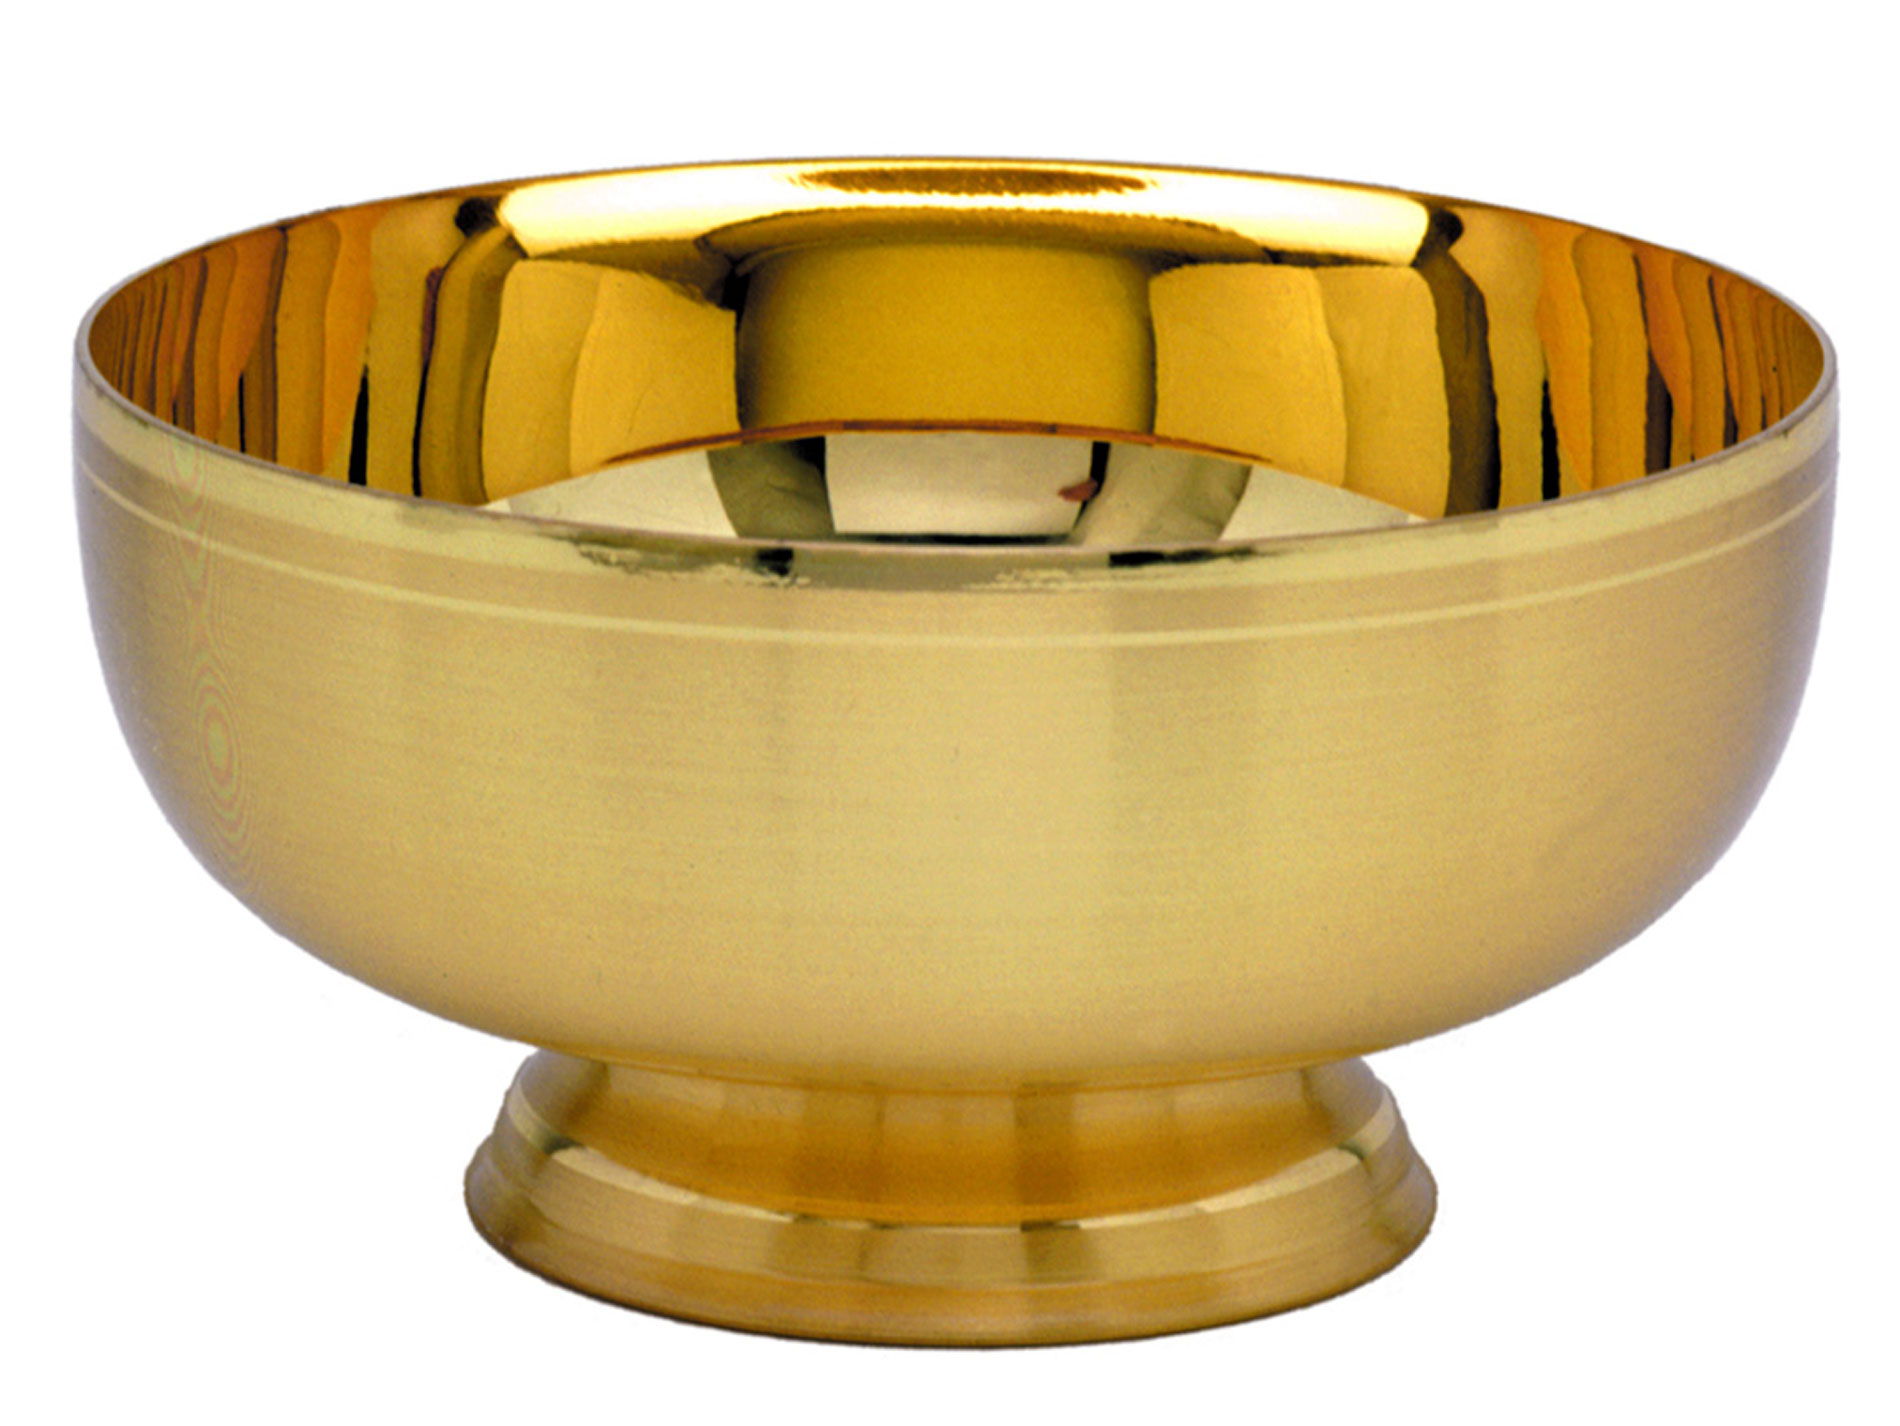
\includegraphics[width=300px]{../img/patena.jpg}
\end{frame}


\end{document}

